\documentclass[10pt]{book}
\usepackage{../styles/print-de}



% Hyperref bitte im main.tex lassen (sollte fast zuletzt geladen werden)
\usepackage{hyperref}
\hypersetup{colorlinks=true, linkcolor=blue, citecolor=teal, urlcolor=magenta}

\begin{document}
	
	% Optional: Titel-/Cover-Seite
	% \begin{titlepage}
		%   \centering
		%   \includegraphics[width=\textwidth]{bilder/cover.png}
		% \end{titlepage}
	
	\hyphenation{exis-tiert}
	
	% Vorwort, ToC
	\cleardoublepage
\thispagestyle{empty}
\begin{center}
	
	{\Large\textbf{Photon – Theory and Applications}}\\[1.2em]
	{\large Dipl.-Ing.\,(FH)\,Christian Weilharter}\\[1.2em]
	\textcopyright~2025, Christian Weilharter, Traunstein\\[2em]
\end{center}

\begin{flushleft}
	\begin{tabular}{@{}l l}
		\textbf{ISBN (Print):} & 978-3-912302-02-8 \\[0.5em]
		\textbf{ISBN (E-Book):} & 978-3-912302-03-5 \\[0.5em]
		\textbf{Edition:} & 1st edition, 2025 \\[0.5em]
		\textbf{Typesetting:} & \LaTeX \\[0.5em]
		\textbf{Publisher:} & Christian Weilharter \\[0.5em]

		\textbf{Print:} & Amazon KDP (Print-on-Demand) \\[0.5em]
		\textbf{E-book edition:} & Apple Books \\[0.5em]
		& Amazon Kindle Direct Publishing \\[0.5em]
		\textbf{Contact:} & \href{mailto:info@mathandphysics.de}{info@mathandphysics.eu} \\[0.5em]
		\textbf{Web:} & \href{https://www.mathandphysics.de}{www.mathandphysics.eu} \\

	\end{tabular}
\end{flushleft}

\vspace{2em}
\noindent
All rights reserved. No part of this book may be reproduced, stored, or transmitted
in any form or by any means, electronic or mechanical, including photocopying,
recording, or by any information storage and retrieval system, without prior written
permission of the author.

\begin{center}\small Printed in Germany\end{center}

\cleardoublepage


\chapter*{Preface}
\markboth{Preface}{Preface} % optional für Kopfzeile
% kein addcontentsline → Preface erscheint NICHT im Inhaltsverzeichnis



The creation of this book has been driven by a deep fascination with light and its fundamental mediator – the photon. In modern physics, the photon plays a central role: as a particle without mass, yet carrying energy and 

\begin{flushright}
	\textit{Dipl.-Ing.(FH) Christian Weilharter} \\
	\vspace{0.5em}
	[Traunstein, 2025]
\end{flushright}

	\tableofcontents
	
	% Hauptkapitel
	\chapter{Einleitung: Warum Mathematik Struktur ist}
\label{chap:I_einfuehrung}

\setlength{\parindent}{0pt}


\subsection{Ausgangsfrage}

Warum brauchen wir überhaupt \textbf{Zahlen}\index{Zahlen}, \textbf{Formen}\index{Formen} und \textbf{Funktionen}\index{Funktionen}, um die Welt zu beschreiben? 
Ist \textbf{Mathematik}\index{Mathematik} nur ein Werkzeug, das Menschen erfunden haben oder steckt dahinter eine tiefere Struktur, die wir entdecken? 
Diese Frage begleitet die gesamte Geschichte der \textbf{Naturwissenschaften}\index{Naturwissenschaften}.
Schon die Griechen erkannten, dass Harmonie – in Musik, Geometrie \index{Geometrie} und sogar im Kosmos \index{Kosmos} – auf Zahlenverhältnissen beruht.
\index{Harmonie}
Später zeigte \textbf{Galileo Galilei}\index{Galilei, Galileo}, dass die Natur „in der Sprache der Mathematik“ geschrieben sei.  
Und bis heute bleibt es erstaunlich, dass abstrakte Symbole, die zunächst nur im Kopf existieren, 
plötzlich die Bahnen von \textbf{Planeten}\index{Planeten}, die Ausbreitung des \textbf{Lichts}\index{Licht} oder die Gesetze der \textbf{Quantenmechanik}\index{Quantenmechanik} beschreiben. 

Die Ausgangsfrage ist also nicht nur theoretisch, sondern berührt unser Bild von der Wirklichkeit: 
Entsteht Mathematik in unserem Denken  oder spiegelt sie eine Ordnung wider, die in der Natur selbst vorhanden ist?


\subsection{Mathematik als universelle Sprache}
\label{sec:1.2_universelle_sprache}

Auffällig ist, dass mathematische Strukturen\index{mathematische Strukturen} 
unabhängig von Kultur\index{Kulturen} und Zeit immer wieder auftauchen. 
Die Griechen\index{Griechen} stießen auf \emph{irrationale Zahlen}\index{irrationale Zahlen}, 
die Inder\index{Indien} erfanden die \emph{Null}\index{Null}, 
arabische Mathematiker\index{arabische Mathematik} entwickelten die \emph{Algebra}\index{Algebra}. 
Trotz unterschiedlicher Sprachen und Traditionen ergibt sich eine gemeinsame innere Logik. 

Besonders bemerkenswert ist, dass verschiedene Kulturen, oft völlig unabhängig voneinander, 
auf dieselben mathematischen Ergebnisse gestoßen sind – sei es bei der 
Berechnung von \emph{Quadratwurzeln}\index{Quadratwurzeln}, 
bei der Entwicklung von \emph{Zahlensystemen}\index{Zahlensysteme} 
oder bei geometrischen Sätzen\index{Geometrie}. 
Dies zeigt: Mathematik ist keine willkürliche Erfindung, sondern eine Struktur, 
die überall entdeckt wird.

Mathematik wirkt wie eine universelle Sprache\index{universelle Sprache}, 
die allen Kulturen zugänglich ist – und die heute gleichermaßen in 
\emph{Informatik}\index{Informatik}, \emph{Quantenphysik}\index{Quantenphysik} 
und \emph{künstlicher Intelligenz}\index{künstliche Intelligenz} sichtbar wird.
\vspace{1em}

\begin{NoteBox}[Unabhängige Entdeckungen]
	Viele Kulturen haben zentrale mathematische Ideen unabhängig voneinander gefunden. 
	Das zeigt: Mathematik ist keine Erfindung, sondern eine Struktur, 
	die überall entdeckt wird.
	\label{box:entdeckung}
\end{NoteBox}

\subsection{Experimente als Schlüssel}

Erst durch \textbf{Experimente}\index{Experimente} zeigte sich, dass diese abstrakten Strukturen in der Natur selbst wirksam sind.
\textbf{Galilei, Galileo}\index{Galilei, Galileo} ließ Kugeln eine schiefe Ebene hinunterrollen und fand: Die Bewegung folgt einer \textbf{Parabel}\index{Parabel}. 
Das \textbf{Thermometer}\index{Thermometer} verdeutlichte die Linearität der Ausdehnung von \textbf{Quecksilber}\index{Quecksilber} – eine gerade Linie im Diagramm. 
\textbf{Ohm, Georg Simon}\index{Ohm, Georg Simon} maß Strom, Spannung und Widerstand und entdeckte die einfache Beziehung \( U = R \cdot I \)\index{Ohmsches Gesetz}. 
Nicht das Denken allein, sondern das Experiment offenbarte diese Gesetzmäßigkeiten.

\subsection{Entdeckung statt Erfindung}

Viele mathematische Konstanten lassen sich nicht willkürlich festlegen. 
Die \textbf{Kreiszahl $\pi$}\index{Kreiszahl $\pi$} ergibt sich zwangsläufig aus der Geometrie des Kreises. 
Die \textbf{Eulersche Zahl $e$}\index{Eulersche Zahl $e$} taucht unvermeidlich in Wachstumsprozessen auf. 
Solche Zahlen und Strukturen sind nicht von Menschen ausgedacht, sondern in der Natur angelegt – wir entdecken sie nur. 
Schon \textbf{Platon}\index{Platon} sah in der Mathematik eine Ideenwelt, die unabhängig vom Menschen existiert. 
Bis heute wird diskutiert, ob Mathematik erfunden oder entdeckt ist – eine Frage, die Philosophie und Naturwissenschaft verbindet.  
\subsection{Fazit}

Die Basis jeder \emph{Mathematik}\index{Mathematik} sind die 
\emph{Zahlen}\index{Zahlen}. 
Von der einfachen \emph{Zählung}\index{Zählen} über 
\emph{irrationale Zahlen}\index{irrationale Zahlen} 
und \emph{negative Zahlen}\index{negative Zahlen} 
bis hin zu \emph{komplexen Zahlen}\index{komplexe Zahlen} zeigt sich: 
Jede Erweiterung eröffnet einen tieferen Blick in die 
\emph{Struktur der Welt}\index{Struktur der Welt}.  

In diesem Buch soll die Hypothese\index{Hypothese} aufgezeigt 
und anhand vieler Beispiele belegt werden, 
dass Mathematik nicht erfunden, sondern \emph{entdeckt}\index{Entdeckung} wurde – 
als universelle Struktur\index{universelle Struktur}, 
die allen \emph{Kulturen}\index{Kulturen} und allen Zeiten\index{Zeit} zugänglich ist.  



\vspace{1em}
\begin{NoteBox}[Zahlen als universale Entdeckung]
	Die Geschichte zeigt: Ob \emph{Babylonier}, \emph{Inder}, \emph{Griechen} oder \emph{Araber} – 
	alle Kulturen stießen auf dieselben mathematischen Strukturen. 
	Den Anfang bilden stets die Zahlen. 
	Darum setzt Kapitel II genau hier an: bei den fundamentalen Bausteinen der Mathematik.
	\label{box:universale}
\end{NoteBox}



	\chapter{Zahlen und Wirklichkeit}
\label{chap:II_zahlen}



% =====================================================
% 2.1 Natürliche Zahlen und Zählen
% =====================================================

\subsection{Natürliche Zahlen und Zählen}
\label{sec:2.1_natuerliche_zahlen}

Die Geschichte der \emph{Zahlen}\index{Zahlen} beginnt mit dem Bedürfnis des Menschen, 
seine Umwelt zu ordnen. 
Lange bevor es \emph{Schrift}\index{Schrift} oder 
\emph{Rechenverfahren}\index{Rechenverfahren} gab, 
nutzte man das \emph{Zählen}\index{Zählen}, um Tiere, Werkzeuge oder Tage festzuhalten. 
Das Zählen war eine grundlegende \emph{Kulturtechnik}\index{Kulturtechnik}, 
ohne die \emph{Handel}\index{Handel}, 
\emph{Planung}\index{Planung} und 
\emph{Wissenschaft}\index{Wissenschaft} 
nicht denkbar gewesen wären.

\subsubsection*{Früheste Ansätze}
\phantomsection
Archäologische Funde\index{Archäologie} deuten darauf hin, dass bereits vor 
rund 20.000 bis 35.000 Jahren \emph{Zählhilfen}\index{Zählhilfen} benutzt wurden. 
Besonders bekannt ist der \emph{Ishango-Knochen}\index{Ishango-Knochen}, 
entdeckt 1960 von Jean de Heinzelin de Braucourt\index{Heinzelin de Braucourt, Jean de} 
in Zentralafrika. 
Noch älter ist das \emph{Lebombo-Knochenstück}\index{Lebombo-Knochen} 
aus Südafrika. Beide Artefakte belegen, dass Menschen schon in der 
\emph{Altsteinzeit}\index{Altsteinzeit} 
mit Einkerbungen Mengen darstellten (vgl.~Abb.~\ref{fig:knochen}). 

\begin{figure}[ht]
	\centering
	\includegraphics[width=0.45\textwidth]{bilder/lebombo-bone.png}
	\hfill
	\includegraphics[width=0.45\textwidth]{bilder/ishango_bone.jpg}
	\caption{Links: Lebombo-Knochenstück (ca.\ 35.000 Jahre alt, Südafrika). 
		Rechts: Ishango-Knochen (ca.\ 20.000 Jahre alt, Zentralafrika). 
		Beide zeigen regelmäßige Einkerbungen, die als frühe Zählhilfen gedeutet werden. 
		Der Ishango-Knochen wird heute im \emph{Königlichen Belgischen Institut für Naturwissenschaften} in Brüssel aufbewahrt.}
	\label{fig:knochen}
\end{figure}



\begin{HistoryBox}[Der Ishango-Knochen]
	Der \emph{Ishango-Knochen} wurde 1960 von 
Jean de Heinzelin de Braucourt in Zentralafrika entdeckt und ist etwa 20.000 Jahre alt. 

Auf dem Knochen finden sich drei Spalten von Einkerbungen, 
die nicht zufällig verteilt sind, sondern in Gruppen geordnet erscheinen. 
Wahrscheinlich diente er als eine Art \emph{Zählstab}\index{Zählstab} – 
möglicherweise zur Beobachtung des \emph{Mondzyklus}\index{Mondzyklus} 
oder zur Zählung von Vorräten.

Besonders auffällig: Einige Gruppierungen entsprechen \emph{Primzahlen}\index{Primzahlen} 
(11, 13, 17, 19). Ob dies Zufall oder Absicht war, bleibt offen. 
Der Knochen zeigt jedoch, dass Menschen schon in der Altsteinzeit 
Zahlen nutzten, um Muster in ihrer Welt zu erkennen und festzuhalten.
\label{box:ishango}
\end{HistoryBox}

Auch andernorts nutzten Menschen Einkerbungen, Knoten oder Steine als einfache Zählhilfen. 
Kerbhölzer dienten über Jahrtausende zur Aufzeichnung von Vorräten, Abgaben oder Schulden – 
bis in die Neuzeit hinein, etwa im Alpenraum. 
Überall griff man unabhängig zur gleichen Idee: 
Einkerbungen als elementare Zählhilfe.

\subsubsection*{Vom Zählen zum Zahlbegriff}
\phantomsection
Neben archäologischen Funden zeigt auch die \emph{Sprachforschung}\index{Sprachforschung}, 
dass Menschen ihre Umwelt zunächst nur grob in kleine und große Mengen unterteilten – 
anfangs: \emph{eins}, \emph{zwei}, \emph{viele}. 

Manche traditionellen Kulturen kennen bis heute nur sehr wenige \emph{Zahlwörter}\index{Zahlen}, 
oft lediglich die Unterscheidung \glqq eins\grqq, \glqq zwei\grqq{} und \glqq viele\grqq, 
etwa in \emph{Papua-Neuguinea}\index{Papua-Neuguinea} oder \emph{Australien}\index{Australien}. 

Das zeigt: \emph{Zahlen}\index{Zahlen} sind keine Selbstverständlichkeit, 
sondern eine kulturelle \emph{Erfindung}, entstanden aus praktischen Bedürfnissen 
wie \emph{Handel}\index{Handel}, \emph{Vorratshaltung}\index{Vorratshaltung} 
oder \emph{Kalenderrechnung}\index{Kalenderrechnung}. 

Überall – in Afrika, Asien, Europa oder Ozeanien – entwickelten Menschen Zählhilfen 
und \emph{Zahlbegriffe}\index{Zahlbegriff}. 
Das Bedürfnis, die Welt in Zahlen zu fassen, spiegelt eine tiefe Struktur der 
\emph{Wirklichkeit}\index{Wirklichkeit} wider.



% =====================================================
% 2.2 Irrationale Zahlen – die Krise der Griechen
% =====================================================

\subsection{Irrationale Zahlen – die Krise der Griechen}
\label{sec:2.2_irrat}

\subsubsection*{Ausgangspunkt: Pythagoras und die Pythagoreer}
\phantomsection
Die frühen griechischen Mathematiker\index{Griechen}, vor allem die Schule der 
\emph{Pythagoreer}\index{Pythagoreer}, waren überzeugt, dass sich die Welt vollständig 
durch \emph{ganze Zahlen}\index{ganze Zahlen} und \emph{Brüche}\index{Brüche} beschreiben lässt. 
Ihr Leitsatz lautete: „Alles ist Zahl.“ 
Der \emph{Satz des Pythagoras}\index{Satz des Pythagoras} war dafür das zentrale Symbol.

\subsubsection*{Erste Erkenntnisse: Inkommensurabilität}
\phantomsection
Beim Quadrat mit Seitenlänge $1$ wollten die Pythagoreer die Länge der Diagonale berechnen. 
Nach dem Satz des Pythagoras gilt:
\[
c^2 = 1^2 + 1^2 = 2 \quad \Rightarrow \quad c = \sqrt{2}.
\]

Die Zahl $\sqrt{2}$ ließ sich jedoch durch keinen Bruch zweier ganzer Zahlen darstellen. 
Damit war klar: Es gibt \emph{inkommensurable Längen}\index{inkommensurabel}, 
die kein gemeinsames Maß besitzen. 
Die Seitenlänge $1$ und die Diagonale $\sqrt{2}$ sind inkommensurabel.
Diese Erkenntnis stellte die Grundüberzeugung der Pythagoreer in Frage, 
dass die Welt ausschließlich durch ganze Zahlen und Brüche erklärbar sei.

\subsubsection*{Die Krise der Griechen}
\phantomsection
Die Entdeckung der Irrationalität stürzte die Pythagoreer in eine intellektuelle Krise.  
Der Überlieferung nach soll \emph{Hippasos von Metapont}\index{Hippasos von Metapont} 
diese Tatsache erkannt haben – 
die Legende berichtet sogar, dass er von seinen Brüdern ertränkt wurde, 
weil er dieses „Geheimnis“ preisgab. 
Ob die Geschichte wahr ist oder nicht: 
Sicher ist, dass die Entdeckung der Irrationalität 
die griechische Mathematik tief erschütterte. 

\subsubsection*{Der Beweis}
\phantomsection
Einen strengen Beweis für die Irrationalität formulierte \emph{Euklid}\index{Euklid} 
im 10.~Buch seiner \emph{Elemente}\index{Elemente (Euklid)}. 
Er basiert auf einem klassischen Widerspruchsargument:



\begin{MathBox}[Widerspruchsbeweis für $\sqrt{2}$]
		Angenommen, $\sqrt{2}$ sei rational, also $\sqrt{2}=\tfrac{p}{q}$ mit 
	ganzen Zahlen $p,q$, die teilerfremd sind. 
	Dann gilt $2q^2=p^2$. 
	Daraus folgt: $p^2$ ist gerade, also ist auch $p$ gerade. 
	Schreiben wir $p=2r$, dann gilt $2q^2=(2r)^2=4r^2$, also $q^2=2r^2$. 
	Damit ist auch $q$ gerade. 
	
	Somit sind $p$ und $q$ beide gerade, also nicht teilerfremd. 
	Dies widerspricht der Annahme. 
	Damit ist $\sqrt{2}$ irrational.
	\label{box:widerspruch}
\end{MathBox}
Anschaulich bedeutet dies: 
Es gibt kein gemeinsames Maß, 
mit dem man gleichzeitig die Seitenlänge $1$ und die Diagonale $\sqrt{2}$ 
genau abmessen könnte. 
Jeder Bruch führt irgendwann in einen Widerspruch. 
$\sqrt{2}$ gehört also nicht zur Welt der Brüche, 
sondern eröffnet die neue Zahlenwelt der \emph{irrationalen Zahlen}\index{irrationale Zahlen}.
Die ausführliche Herleitung des Beweises findet sich in 
Anhang~\ref{anhangA_wurzel2}.

\subsubsection*{Näherungen und Berechnung}
\phantomsection
Trotz der Irrationalität blieb $\sqrt{2}$ unverzichtbar. 
Darum entwickelten verschiedene Kulturen Verfahren, den Wert möglichst genau zu bestimmen.

\subsubsection*{Indische Näherung (Śulba-Sūtras).}
\phantomsection
In den altindischen \emph{Śulba\-/Sūtras}\index{Śulba-Sūtras}\index{Indien!Mathematik}
findet sich eine berühmte Näherungsregel für $\sqrt{2}$:
\[
\sqrt{2}\approx 1+\frac{1}{3}+\frac{1}{3\cdot 4}\;-\;\frac{1}{3\cdot 4\cdot 34}
\;=\;1.414\,215\ldots
\]
Schon sechs Nachkommastellen stimmen mit dem exakten Wert überein.

\subsubsection*{Griechische Verfahren: Iteration und Kettenbruch.}
\phantomsection
Arithmetisch nutzten die Griechen das Verfahren 
$x_{n+1}=\tfrac{1}{2}(x_n+\tfrac{2}{x_n})$, 
das rasch zu $\sqrt{2}$ konvergiert – 
heute bekannt als \emph{Newton-Verfahren}.  
Geometrisch wurde die sogenannte \emph{Anthyphairesis} verwendet, 
eine frühe Form des Kettenbruchs:
\[
\sqrt{2}=[1;\overline{2}]=1+\cfrac{1}{2+\cfrac{1}{2+\cdots}}
\]
Die Konvergenten ($3/2,\ 7/5,\ 17/12,\dots$) liefern immer bessere Bruchnäherungen; 
das periodische Muster $\overline{2}$ macht die Irrationalität sichtbar.


\begin{NoteBox}[Mathematik als Entdeckung]
	Die Entdeckung der irrationalen Zahlen war ein Wendepunkt: 
	Zahlen sind keine bloßen Erfindungen, sondern beschreiben Strukturen, 
	die in der Natur tatsächlich vorkommen. 
	Das Quadrat mit Seitenlänge $1$ „erzwingt“ die Existenz von $\sqrt{2}$.
	\label{box:mathentdeckung}
\end{NoteBox}
% =====================================================
% 2.3 Null und negative Zahlen
% =====================================================

\subsection{Null und negative Zahlen}
\label{sec:2.3_null_negative}

\subsubsection*{Einleitung}
\phantomsection
Die Vorstellung von \emph{Nichts}\index{Nichts} als Zahl und die Idee von \emph{negativen Zahlen}\index{negative Zahlen} 
sind für uns heute selbstverständlich. 
Historisch jedoch war ihre Entwicklung lang und von Widerständen begleitet. 
Für viele Kulturen war es kaum vorstellbar, 
dass es eine Zahl für „nichts“ geben sollte – oder gar für „weniger als nichts“. 

\subsubsection*{Die Null – Zahl aus dem Nichts}
\phantomsection
Schon die Babylonier nutzten ein Platzhaltersymbol, wenn eine Stelle leer blieb. 
Eine wirkliche \emph{Null als Zahl} entwickelte sich jedoch erst in Indien.  
Dort formulierte \textbf{Brahmagupta}\index{Brahmagupta} im Jahr 628 n.\,Chr. erstmals Rechenregeln mit $0$ 
(in seinem \emph{Brahmasphutasiddhanta}).  
Über die arabische Welt gelangte das Konzept nach Europa und wurde 
durch \textbf{Leonardo Fibonacci}\index{Fibonacci, Leonardo} in seinem \emph{Liber Abaci} (1202) verbreitet.

Viele Philosophen und Theologen taten sich mit der Null schwer. 
Wie konnte „Nichts“ eine Zahl sein? 
In Europa galt sie lange als verdächtig oder sogar gefährlich, 
da sie mit der Idee des Abgrunds oder des Nichtseins verbunden war.  
Heute ist die Null Grundlage des Stellenwertsystems und 
unverzichtbar für die moderne Mathematik.

\subsubsection*{Negative Zahlen – Schulden und Temperaturen}
\phantomsection
Negative Zahlen tauchten bereits in China um 200 v.\,Chr. auf, 
in den \emph{Neun Büchern über die Mathematik}\index{China!Neun Bücher über die Mathematik}.  
Man unterschied positive und negative Werte mit verschiedenfarbigen Rechenstäbchen: 
rot für Gewinne, schwarz für Verluste.  
Auch in Indien wurden negative Zahlen verwendet, etwa zur Darstellung von Schulden oder Defiziten. 

\begin{figure}[ht]
	\centering
	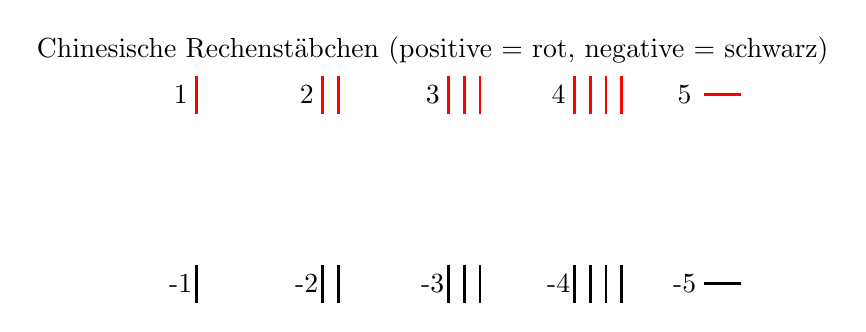
\begin{tikzpicture}[scale=0.8, line width=1pt]
		\node at (4,3.2) {Chinesische Rechenstäbchen (positive = rot, negative = schwarz)};
		% Positive Zahlen (rot)
		\foreach \n/\count in {1/1, 2/2, 3/3, 4/4} {
			\node at (2*\n-2,2.5) {\n};
			\foreach \i in {1,...,\count} {
				\draw[red] (2*\n-2+0.25*\i,2.2) -- (2*\n-2+0.25*\i,2.8);
			}
		}
		\node at (8,2.5) {5};
		\draw[red] (8.3,2.5) -- (8.9,2.5);
		% Negative Zahlen (schwarz)
		\foreach \n/\count in {1/1, 2/2, 3/3, 4/4} {
			\node at (2*\n-2,-0.5) {-\n};
			\foreach \i in {1,...,\count} {
				\draw[black] (2*\n-2+0.25*\i,-0.8) -- (2*\n-2+0.25*\i,-0.2);
			}
		}
		\node at (8,-0.5) {-5};
		\draw[black] (8.3,-0.5) -- (8.9,-0.5);
	\end{tikzpicture}
	\caption{Chinesische Rechenstäbchen: positive Zahlen (rot), negative Zahlen (schwarz).}
	\label{fig:rod_numerals_colored}
\end{figure}


\begin{MathBox}[Rechenregeln für negative Zahlen]
Heute sind die Regeln vertraut:
\[
(+a)+(-b)=a-b, \quad (-a)+(-b)=-(a+b),
\]
\[
(-a)\cdot(-b)=+ab, \quad (-a)\cdot b=-(ab).
\]
Doch diese einfachen Regeln wurden in Europa erst sehr spät akzeptiert. 
\textbf{René Descartes}\index{Descartes, René} bezeichnete negative Zahlen noch als 
„falsche Zahlen“.
\label{box:negative}
\end{MathBox}


Viele Mathematiker fragten sich: 
Wie kann man „weniger als nichts“ besitzen? 
Ein negatives Ergebnis schien absurd. 
Erst durch praktische Anwendungen wie Buchhaltung (Schulden) oder 
Temperaturmessungen unter Null wurde ihre Nützlichkeit offensichtlich.
Mit der Null und den negativen Zahlen erweiterte sich das Zahlensystem entscheidend: 
Mathematik begann, nicht nur das Zählen von Dingen zu beschreiben, 
sondern auch Abwesenheit und Gegensätze. 
So entstand die moderne Zahlengerade, 
auf der sich alle ganzen Zahlen von $-\infty$ bis $+\infty$ anordnen lassen.

% =====================================================
% 2.4 Komplexe Zahlen – eine unerwartete Erweiterung
% =====================================================

\subsection{Komplexe Zahlen – eine unerwartete Erweiterung}
\label{sec:2.4_komplexe}

\subsubsection*{Einleitung}
\phantomsection
Während Brüche, irrationale Zahlen, die Null und die negativen Zahlen jeweils aus praktischen 
Problemen hervorgegangen sind, entstand die nächste Erweiterung des Zahlbegriffs fast beiläufig: 
die sogenannten \emph{komplexen Zahlen}.  
Sie tauchten auf, als man versuchte, Gleichungen zu lösen, 
die mit den bekannten Zahlenarten nicht lösbar waren.

\subsubsection*{Erste Ansätze in der Renaissance}
\phantomsection
Im 16.~Jahrhundert beschäftigten sich italienische Mathematiker wie 
\textbf{Scipione del Ferro}\index{del Ferro, Scipione}, 
\textbf{Niccolò Tartaglia}\index{Tartaglia, Niccolò} und 
\textbf{Gerolamo Cardano}\index{Cardano, Gerolamo} mit kubischen Gleichungen.  
Bei manchen Lösungswegen traten Zwischenschritte mit $\sqrt{-1}$ auf – 
obwohl das Endergebnis wieder eine reelle Zahl war.  
Cardano nannte diese Ausdrücke „sophistische Wurzeln“ – 
er schrieb sie zwar auf, verstand sie aber nicht.  
Man hielt sie für eine Art Rechenkuriosität: notwendig im Lösungsweg, 
aber ohne eigenständige Bedeutung.

\subsubsection*{Bombelli und die Wende}
\phantomsection
Der italienische Mathematiker \textbf{Rafael (Raffaele) Bombelli}\index{Bombelli, Rafael} erkannte um 1572, 
dass man mit diesen „imaginären Zahlen“ konsistent rechnen kann, 
wenn man sie wie gewöhnliche Zahlen behandelt und $i^2=-1$ setzt.  
Damit legte er den Grundstein für die Theorie der komplexen Zahlen.

Noch lange galten komplexe Zahlen als „fiktiv“ oder „imaginär“.  
Erst im 18.~und 19.~Jahrhundert, bei \textbf{Leonhard Euler}\index{Euler, Leonhard}, 
\textbf{Carl Friedrich Gauss}\index{Gauss, Carl Friedrich} und 
\textbf{Jean-Robert Argand}\index{Argand, Jean-Robert}, 
setzte sich die Erkenntnis durch:  
Komplexe Zahlen sind nicht nur Hilfsmittel, sondern eine 
notwendige und vollwertige Erweiterung des Zahlbegriffs.  

\subsubsection*{Bedeutung}
\phantomsection
Heute bilden die komplexen Zahlen ein Fundament der modernen Mathematik.  
Sie garantieren mit dem \emph{Fundamentalsatz der Algebra}\index{Fundamentalsatz der Algebra}, 
dass jedes Polynom eine Lösung besitzt, 
und sind in Physik und Technik unverzichtbar – etwa für Schwingungen, Wellen, 
Quantenmechanik und Elektrotechnik.

Die ausführliche historische Herleitung und die formale Einführung von $i^2=-1$ 
finden sich im Anhang~\ref{anhangA_komplexe}.

% =====================================================
% 2.5 Fazit
% =====================================================

\subsection{Fazit: Zahlen als entdeckte Struktur}

Vom Zählen der Herden bis zur Einführung der komplexen Zahlen zeigt sich ein roter Faden: 
Neue Zahlenarten entstehen nicht willkürlich, sondern immer dann, wenn die bisherigen 
Zahlen nicht mehr ausreichen.  

\begin{itemize}
	\item Die \emph{natürlichen Zahlen}\index{natürliche Zahlen} entstanden aus dem praktischen Bedürfnis zu zählen.  
	\item \emph{Irrationale Zahlen}\index{irrationale Zahlen} wurden entdeckt, als die Geometrie den Bereich der Brüche sprengte.  
	\item Die \emph{Null}\index{Null} und die \emph{negativen Zahlen}\index{negative Zahlen} öffneten den Blick für Abwesenheit und Gegensätze.  
	\item Die \emph{komplexen Zahlen}\index{komplexe Zahlen} machten scheinbar unlösbare Gleichungen lösbar und führten zur Vollständigkeit der Mathematik.  
\end{itemize}


\begin{NoteBox}[Zahlen als universelle Struktur]
	Zahlen sind keine freie Erfindung des Menschen.  
	Sie wurden Schritt für Schritt \emph{entdeckt}, weil die Welt selbst 
	eine innere Struktur hat, die wir in Zahlen fassen können.  
	Durch logisches Weiterdenken und konsequentes Rechnen erschlossen sich immer neue Zahlbereiche – 
	von den Kerben auf Knochen bis hin zur komplexen Ebene.  
	\label{box:universelle}
\end{NoteBox}
	
\chapter{Algebra und Gleichungen}
\label{chap:III_algebra}
\label{chap:III_qubit}
\setcounter{section}{3}
\setcounter{subsection}{0}
\setcounter{subsubsection}{1}
\setcounter{secnumdepth}{3}
\subsection{Die arabische Mathematik und die Geburt der Algebra}
\label{sec:3.1_arabische_mathematik}

Nach den Griechen, Indern und Babyloniern war es die arabisch-islamische Welt, 
die die Mathematik auf eine neue, systematische Ebene hob. 
Während in Europa das antike Wissen weitgehend verloren ging, 
bewahrten und erweiterten Gelehrte wie 
\emph{al-Chwarizmi}\index{al-Chwarizmi, Muhammad ibn Musa}, 
\emph{Omar Chayyām}\index{Chayyām, Omar} und 
\emph{al-Karaji}\index{al-Karaji, Abu Bakr} die Erkenntnisse ihrer Vorgänger. 

Im 9.~Jahrhundert verfasste \emph{al-Chwarizmi} in Bagdad das Werk 
\emph{„Kitāb al-jabr wa’l-muqābala“}\index{Kitāb al-jabr wa’l-muqābala}, 
das als Geburtsstunde der \emph{Algebra}\index{Algebra} gilt. 
Der Begriff „al-jabr“ bedeutet sinngemäß „das Wiederherstellen“ oder „das Ergänzen“, 
„al-muqabala“ bezeichnet „das Gegenüberstellen“. 
Gemeint war damit eine Methode, Unbekanntes zu isolieren und Gleichungen zu vereinfachen – 
eine Revolution im Denken über Zahlen und Formen. 


\begin{HistoryBox}[Von der Praxis zur Theorie]
Im Mittelpunkt der arabischen Mathematik stand anfangs die Lösung praktischer Probleme: 
Verteilung von Erbschaften, Berechnung von Grundstücksflächen, 
Bestimmung von Handelsanteilen oder astronomische Messungen. 
Doch aus diesen konkreten Aufgaben entwickelte sich ein allgemeines Verfahren, 
Unbekannte zu bestimmen – die Geburt der symbolischen Methode.
\label{box:praxis}
\end{HistoryBox}
Ein klassisches Beispiel aus der frühen arabischen Mathematik ist die Berechnung von Erbanteilen. 
Nach islamischem Recht erhält eine Frau den achten Teil des Nachlasses, 
der Rest wird unter den Söhnen gleich verteilt. 
Beträgt das Erbe insgesamt 600~Dinar, so ergibt sich:

\[
1 = \tfrac{1}{8} + 2x,
\]
wobei \(x\) den Anteil eines Sohnes beschreibt. 
Nach Umformen folgt \(x = \tfrac{7}{16}\). 
Damit erhält jeder Sohn \(x \cdot 600 = 262{,}5\)~Dinar, 
die Frau \(75\)~Dinar.
\begin{HistoryBox}[Vom praktischen Problem zur abstrakten Gleichung]
	Die arabischen Mathematiker formulierten solche Beziehungen symbolisch 
	und lösten sie durch \emph{al-jabr} (Ergänzen) und \emph{al-muqabala} (Gegenüberstellen). 
	So entstand aus einem alltäglichen Rechenproblem die Idee der allgemeinen Gleichung – 
	der Beginn der Algebra als abstraktes Denken.
	\label{box:abstrakten}
\end{HistoryBox}

\begin{NoteBox}[Ein gemeinsames Erbe]
	Die arabischen Mathematiker erfanden die Algebra nicht aus dem Nichts. 
Sie knüpften an das Wissen der Babylonier, Griechen und Inder an. 
Schon die Babylonier lösten Gleichungen der Form \(x^2 + bx = c\) 
mit tabellarischen Methoden, und die Griechen beschrieben geometrische Zusammenhänge, 
die im Kern algebraisch waren. 
In Indien entstanden symbolische Rechenverfahren für Unbekannte (\emph{yāvattavat}). 
Die arabischen Gelehrten verbanden all diese Traditionen, 
gaben ihnen eine einheitliche Sprache und machten daraus ein geschlossenes System – 
die \emph{Al-jabr}, die wir heute Algebra nennen.
\label{box:erbe}
\end{NoteBox}




Ein bekanntes Beispiel aus Al-Chwarizmis Werk lautet:
\begin{quote}
	„Ein Quadrat und zehn seiner Wurzeln ergeben neununddreißig.“
\end{quote}
Heute würden wir dies als
\[
x^2 + 10x = 39
\]
schreiben.  
Al-Chwarizmi dachte jedoch geometrisch: Das Glied \(x^2\) stellte ein Quadrat dar, 
dessen Seitenlänge \(x\) ist. Die Terme \(10x\) bildeten zwei Rechtecke der Breite~5, 
die an zwei Seiten des Quadrats anliegen.  
Das fehlende kleine Quadrat in der Ecke, das die Figur zu einem größeren Quadrat ergänzt, 
hat die Fläche \(5^2 = 25\).  
Durch Hinzufügen dieser Fläche wird das Gebilde zu einem vollständigen Quadrat:
\[
x^2 + 10x + 25 = 39 + 25,
\]
also \((x+5)^2 = 64\), woraus \(x = 3\) folgt.
\subsubsection*{Graphische Darstellung der quadratischen Ergänzung}
\phantomsection
\begin{figure}[h!]
	\centering
	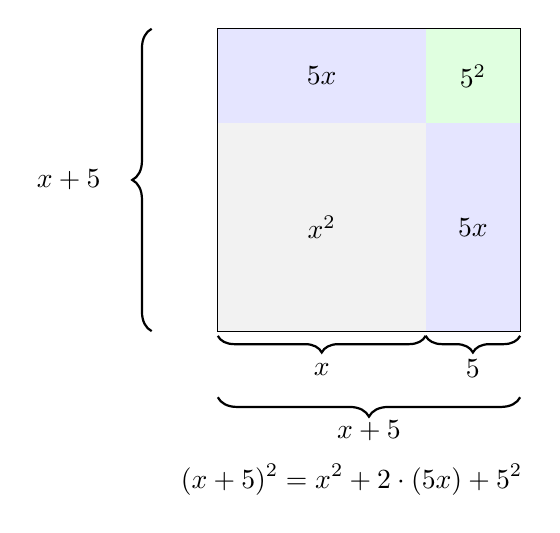
\begin{tikzpicture}[scale=0.12, thick]
		\def\xlen{22}   % Länge x (grafisch)
		\def\five{10}   % Länge 5  (grafisch)
		
		% Gesamtquadrat (x+5)
		\draw (0,0) rectangle (\xlen+\five,\xlen+\five);
		
		% Unterteilung
		\draw (\xlen,0) -- (\xlen,\xlen+\five);
		\draw (0,\xlen) -- (\xlen+\five,\xlen);
		
		% Füllungen
		\fill[gray!10] (0,0) rectangle (\xlen,\xlen);                 % x^2
		\fill[blue!10] (0,\xlen) rectangle (\xlen,\xlen+\five);       % 5x (oben)
		\fill[blue!10] (\xlen,0) rectangle (\xlen+\five,\xlen);       % 5x (rechts)
		\fill[green!12] (\xlen,\xlen) rectangle (\xlen+\five,\xlen+\five); % 5^2
		
		% Beschriftungen
		\node at ({\xlen/2},{\xlen/2}) {$x^2$};
		\node at ({\xlen/2},{\xlen+\five/2}) {$5x$};
		\node at ({\xlen+\five/2},{\xlen/2}) {$5x$};
		\node at ({\xlen+\five/2},{\xlen+\five/2}) {$5^2$};
		
		% Nur eine geschweifte Klammer unten (5 dann x)
	%	\draw [decorate, decoration={brace, amplitude=6pt}]
	%	(0,-2) -- (\five,-2) node[midway, yshift=-10pt] {$5$};
		\draw [decorate, decoration={brace, amplitude=6pt,mirror}]
		(0,-0.5) -- (\xlen,-0.5) node[midway, yshift=-12pt] {$x$};
			\draw [decorate, decoration={brace, amplitude=6pt,mirror}]
		(\xlen,-0.5) -- (\xlen+10,-0.5) node[midway, yshift=-12pt] {$5$};
		% Gesamtlänge unten (x+5)
		\draw [decorate, decoration={brace, amplitude=7pt,mirror}]
		(0,-7) -- (\xlen+\five,-7) node[midway, yshift=-12pt] {$x+5$};
		
		% Linke Gesamtlänge (optional, schmal)
		\draw [decorate, decoration={brace, amplitude=7pt}]
		(-7,0) -- (-7,\xlen+\five) node[midway, xshift=-30pt] {$x+5$};
		
		% Titel
		\node[below right] at (-5,\xlen+\five-45)
		{$\displaystyle (x+5)^2 = x^2 + 2\cdot(5x) + 5^2$};
	\end{tikzpicture}
	\caption{Aus den Teilflächen $x^2$, $5x$ und $5^2$ entsteht das Quadrat $(x+5)^2$.}
\end{figure}





Diese geometrische Methode des Ergänzens – das eigentliche „al-jabr“ – 
führte direkt zur allgemeinen Regel für quadratische Gleichungen, 
die wir heute in symbolischer Form schreiben.  


\begin{DidacticBox}[Der Ursprung des Wortes „Algorithmus“]
	Der Name \emph{al-Chwarizmi} wurde im Lateinischen zu „Algoritmi“ verfremdet. 
Daraus entstand das Wort \emph{Algorithmus}\index{Algorithmus}. 
Damit geht auch ein zweiter Grundpfeiler der modernen Mathematik 
– die systematische, regelhafte Berechnung – 
auf die arabische Wissenschaft zurück.
\label{box:ursprung}
\end{DidacticBox}
Die Algebra war also weniger eine Entdeckung im modernen Sinn, 
sondern eine geistige Neuordnung des vorhandenen Wissens. 
Sie verband die indischen Zahlensysteme mit griechischer Geometrie 
und formte daraus ein allgemeines Rechenverfahren. 
Damit begann die Mathematik, ihre eigene Sprache zu entwickeln – 
eine Sprache der Symbole, Regeln und Abstraktionen.

\subsection{Gleichungen als Werkzeuge zur Problemlösung}
Gleichungen wurden zum universellen Werkzeug, um unbekannte Größen zu berechnen. 
Von einfachen linearen Gleichungen bis zu quadratischen Formen zeigte sich ihre enorme Nützlichkeit. 

\subsection{Die Entstehung der komplexen Zahlen}
Bei der Lösung höherer Gleichungen traten scheinbar „unmögliche“ Zahlen auf. 
Aus dieser Notwendigkeit heraus entstanden die komplexen Zahlen, die bald eine tiefe Bedeutung erhielten. 

\subsection{Mathematik als System von Regeln}
Mit Algebra und Gleichungen begann die Mathematik, sich stärker als ein in sich geschlossenes Regelwerk zu verstehen. 
Diese Sichtweise prägte die weitere Entwicklung bis in die Moderne. 

	\chapter{Mathematik als Sprache der Natur}
\label{chap:IV_sprache}
\label{chap:IV_algorithmen}
\setcounter{section}{4}
\setcounter{subsection}{0}
\setcounter{subsubsection}{1}
\setcounter{secnumdepth}{3}
\setlength{\parindent}{0pt}


\subsection{Galilei und die neue Physik}
\textbf{Galilei}\index{Galilei, Galileo} erkannte, dass die Naturgesetze mathematisch formulierbar sind. 
Seine Experimente mit fallenden Körpern machten deutlich: Bewegung folgt klaren Regeln, die sich in Gleichungen ausdrücken lassen. 

\subsection{Funktionen und Bewegungsgesetze}
Mit dem Begriff der \textbf{Funktion}\index{Funktion} konnten Zusammenhänge präzise beschrieben werden. 
Ob Geschwindigkeit, Kraft oder Energie – in jedem Fall wurde eine mathematische Form die Sprache der Natur. 

\subsection{Differentialgleichungen und Wachstum}
Die Einführung der \textbf{Differentialgleichungen}\index{Differentialgleichung} eröffnete neue Möglichkeiten. 
Von der Mechanik über die Himmelskörper bis hin zu Wachstumsprozessen ließen sich Entwicklungen nun systematisch erfassen. 

\subsection{Von der Mechanik zur modernen Physik}
Die Sprache der Mathematik blieb nicht auf die klassische Mechanik beschränkt. 
Auch Elektrodynamik, Relativitätstheorie und Quantenphysik beruhen auf denselben Prinzipien – 
die Natur spricht überall dieselbe Sprache. 

 \chapter{The Photon in Quantum Electrodynamics (QED)}
\setcounter{section}{5}
\setcounter{subsection}{0}
\setcounter{subsubsection}{1}
\setcounter{secnumdepth}{3}
\setlength{\parindent}{0pt}


\subsection{From the Photon to Quantum Electrodynamics}

The
	\chapter{Zufall -- Eigenschaft der Welt oder Grenze unserer Beschreibung?}
\index{Zufall}





\subsection{Einleitung}

Im Alltag begegnet uns der Zufall auf Schritt und Tritt. Ein Würfel fällt auf eine bestimmte Zahl, das Wetter ändert sich unerwartet, Krankheiten treten scheinbar ohne Ursache auf. Zufall gilt als das Gegenstück zur Ordnung: als Ausdruck von Beliebigkeit, Unvorhersagbarkeit oder fehlender Struktur. Wo Zufall herrscht, so scheint es, versagt jede Gesetzmäßigkeit.

Gleichzeitig ist es gerade die Mathematik, die dem Zufall eine präzise Form gibt. Wahrscheinlichkeiten lassen sich berechnen\index{Wahrscheinlichkeit}, Häufigkeiten vorhersagen, statistische Gesetze formulieren\index{Statistik}. Paradoxerweise entsteht ausgerechnet dort Ordnung, wo der Zufall regiert. Große Zahlen gehorchen stabilen Regeln\index{Gesetz der grossen Zahlen}, Mittelwerte verhalten sich zuverlässig, und viele Naturgesetze gelten nicht für einzelne Ereignisse, sondern nur im statistischen Sinn\index{Naturgesetz}.

Diese Spannung führt zu einer grundlegenden Frage: Ist Zufall eine echte Eigenschaft der Welt – oder lediglich ein Ausdruck unserer begrenzten Beschreibungsmöglichkeiten?

In der klassischen Physik schien die Antwort lange klar. Kennt man die Anfangsbedingungen eines Systems exakt, so ist seine Zukunft eindeutig festgelegt\index{Determinismus}. Zufall erscheint hier lediglich als Folge von Unwissen, Messungenauigkeit oder praktischer Unmöglichkeit. Die Welt selbst bleibt strikt determiniert.

Doch mit dem Aufkommen moderner Physik verschiebt sich dieses Bild. In der Thermodynamik treten Gesetze auf, die nur im Mittel gelten\index{Thermodynamik}. In der Chaostheorie zeigen einfache, deterministische Systeme ein Verhalten, das praktisch nicht vorhersagbar ist\index{Chaostheorie}. Und in der Quantenmechanik scheint der Zufall selbst einen fundamentalen Platz einzunehmen – nicht als Mangel an Wissen, sondern als konstitutives Element der Naturbeschreibung\index{Quantenmechanik}.

Dieses Kapitel untersucht, was wir unter \glqq Zufall\grqq{} tatsächlich verstehen, wie die Mathematik ihn formalisiert und welche Rolle er in den Naturwissenschaften spielt. Dabei geht es nicht um technische Details oder Berechnungen, sondern um das begriffliche Fundament: um die Frage, ob Zufall zur Struktur der Welt gehört oder an den Grenzen unserer Erkenntnis entsteht.

Am Ende wird sich zeigen, dass Zufall kein Gegenbegriff zur Ordnung ist. Vielmehr offenbart er eine tiefere Ebene mathematischer Struktur\index{Struktur} – eine Ordnung, die nicht im einzelnen Ereignis liegt, sondern im Ganzen sichtbar wird.
\begin{NoteBox}[Leitfrage und roter Faden]
	\small
	\begin{itemize}
		\item \textbf{Leitfrage:} Ist Zufall eine Eigenschaft der Welt – oder ein Name für unsere Grenzen?
		\item \textbf{Schlüsselidee:} Mathematik macht Zufall nicht \glqq weg\grqq{}, sondern \emph{formalisierbar}.
		\item \textbf{These dieses Kapitels:} Ordnung zeigt sich nicht im einzelnen Ereignis, sondern in den
		\emph{statistischen Strukturen} des Ganzen.
	\end{itemize}
\end{NoteBox}
\index{Statistik}
\subsection{Würfel und die Entstehung der Wahrscheinlichkeitstheorie}
\index{Zufall}
\index{Würfel}

Der Würfel gilt als eines der ältesten und anschaulichsten Symbole des Zufalls. Seit Jahrhunderten dient er in Spielen, Losverfahren und Experimenten als Sinnbild für Unvorhersagbarkeit. Jeder einzelne Wurf scheint offen: Jede Augenzahl kann auftreten, ohne dass sich vorhersagen ließe, welche es sein wird. In dieser Perspektive erscheint der Zufall als Inbegriff von Beliebigkeit.

Gleichzeitig ist der Würfel ein streng konstruiertes Objekt. Seine Seiten sind gleich groß, seine Form hochsymmetrisch, seine möglichen Ergebnisse klar begrenzt. Nichts an ihm ist chaotisch oder ungeordnet. Der Zufall entsteht nicht aus einem Mangel an Struktur, sondern gerade aus einer wohldefinierten Ausgangslage. Diese Spannung macht den Würfel zu einem idealen Denkmodell für das Verständnis von Zufall.

Wird ein Würfel nur einmal geworfen, bleibt das Ergebnis unvorhersagbar. Wird er jedoch viele Male geworfen, zeigt sich ein überraschendes Phänomen: Die Häufigkeiten der einzelnen Augenzahlen beginnen sich zu stabilisieren. Keine Zahl verschwindet, keine dominiert dauerhaft. Mit wachsender Anzahl von Würfen nähert sich das Gesamtbild einer festen Verteilung an. Ordnung entsteht nicht trotz des Zufalls, sondern durch seine Wiederholung.
\index{Häufigkeit}
\index{Wahrscheinlichkeit}

\begin{DidacticBox}[Einzelwurf vs. Gesetz im Ganzen]
	\small
	\textbf{Wichtige Unterscheidung:}
	\begin{itemize}
		\item Der \textbf{einzelne} Wurf bleibt prinzipiell unvorhersagbar.
		\item Erst eine \textbf{lange Serie} zeigt stabile Muster: relative Häufigkeiten nähern sich einer Verteilung.
		\item \textbf{Wahrscheinlichkeit} ist daher keine Aussage über den nächsten Wurf, sondern über das
		\textbf{Verhalten vieler Wiederholungen}.
	\end{itemize}
\end{DidacticBox}

Diese Beobachtung markiert den gedanklichen Ursprung der Wahrscheinlichkeitstheorie. Ausgangspunkt waren nicht abstrakte mathematische Probleme, sondern sehr konkrete Fragen aus dem Bereich des Glücksspiels: Wie fair ist ein Spiel? Welche Einsätze sind gerechtfertigt? Erst durch die systematische Betrachtung vieler gleichartiger Zufallsexperimente wurde deutlich, dass sich Zufall mathematisch fassen lässt. Die Mathematik erfand den Zufall nicht – sie entdeckte seine Struktur.
\index{Wahrscheinlichkeitstheorie}
\index{Mathematisierung}

Entscheidend ist dabei ein Perspektivwechsel. Wahrscheinlichkeitsaussagen beziehen sich nicht auf das einzelne Ereignis. Sie sagen nichts darüber aus, welche Zahl beim nächsten Wurf erscheinen wird. Stattdessen beschreiben sie Eigenschaften von Gesamtheiten: von langen Reihen gleichartiger Versuche. Der Zufall bleibt bestehen, erhält aber eine präzise Bedeutung.
\index{Gesetz}
\index{Struktur}

Zufall und Gesetzmäßigkeit stehen damit nicht im Widerspruch. Der einzelne Wurf bleibt unvorhersagbar, während die Gesamtheit einer klaren Ordnung folgt. Diese Einsicht ist grundlegend für alle späteren Anwendungen der Wahrscheinlichkeitstheorie. Sie bereitet den Weg zu einer Naturbeschreibung, in der Gesetze nicht mehr jedes einzelne Ereignis festlegen, sondern nur noch das statistische Verhalten vieler Systeme bestimmen.
\index{Statistik}
\index{Naturbeschreibung}

\begin{NoteBox}[Praxis-Test: Ordnung aus vielen Würfen]
	\small
	Die Idee ist simpel: \textbf{Nicht} das einzelne Ereignis erklärt die Struktur, sondern die Statistik.
	Ein konsequent durchgeführtes Würfel-Experiment zeigt anschaulich:
	\begin{itemize}
		\item Abweichungen sind normal – aber sie \textbf{relativieren sich} mit wachsender Datenmenge.
		\item Was wie Beliebigkeit wirkt, wird im Ganzen zu einer \textbf{messbaren Ordnung}.
	\end{itemize}
\end{NoteBox}

Ein besonders eindrückliches Beispiel stammt aus dem persönlichen Bericht eines Physikers, der in der Quantenmechanik tätig war. Trotz seiner theoretischen Vertrautheit mit Wahrscheinlichkeiten und statistischen Gesetzen wollte er sich mit der rein abstrakten Erklärung nicht zufriedengeben. Um die Vorhersagen der Wahrscheinlichkeitstheorie selbst zu überprüfen, entschloss er sich zu einem einfachen, aber konsequenten Experiment: Er würfelte – nicht einige Male, sondern tausende Male.

Mit zunehmender Anzahl der Würfe zeigte sich genau das Verhalten, das die Theorie vorhersagt. Jede der sechs Augenzahlen trat nahezu gleich häufig auf, Abweichungen vom idealen Erwartungswert wurden mit wachsender Datenmenge immer kleiner. Das einzelne Ereignis blieb unvorhersagbar, doch das Gesamtbild erwies sich als bemerkenswert stabil.

Für den Physiker war das weniger eine Bestätigung bekannter Formeln als eine Erfahrung: Statistik ist keine Intuition, sondern eine Ordnung, die erst im Ganzen sichtbar wird.
\index{Wahrscheinlichkeit}
\index{Statistik}
\subsection{Statistik und Naturgesetze}
\index{Statistik}
\index{Naturgesetz}

In vielen Bereichen der Naturwissenschaften treten Gesetze nicht als exakte Vorschriften für einzelne Ereignisse auf, sondern als statistische Regelmäßigkeiten. Im Alltag erwartet man oft, ein Naturgesetz müsse jedes Detail eindeutig festlegen. In der Praxis zeigt sich jedoch: Viele Aussagen der Physik gelten erst \emph{im Mittel} über eine große Anzahl von Einzelfällen hinweg.

Ein klassisches Beispiel liefert die Beschreibung von Gasen. Ein einzelnes Gasteilchen bewegt sich unregelmäßig, stößt mit anderen Teilchen zusammen und ändert ständig Richtung und Geschwindigkeit. Sein konkreter Bewegungsablauf ist weder vollständig messbar noch praktisch vorhersagbar. Dennoch lassen sich für große Gasmengen äußerst präzise Gesetze formulieren, etwa für Druck, Temperatur oder Volumen. Diese Größen beschreiben nicht das Verhalten einzelner Teilchen, sondern statistische Eigenschaften des Gesamtsystems.
\index{Thermodynamik}

Hier zeigt sich ein grundlegendes Prinzip: Je größer die Zahl der beteiligten Elemente, desto stabiler werden statistische Aussagen. Zufällige Schwankungen einzelner Teilchen mitteln sich aus, und das System als Ganzes folgt klaren, reproduzierbaren Gesetzmäßigkeiten. Die Ordnung liegt nicht im Detail, sondern im Kollektiv.
\index{Gesetz}
\index{Kollektiv}

Diese Art von Gesetzmäßigkeit unterscheidet sich vom klassischen Ideal des Determinismus. Naturgesetze beschreiben dann nicht mehr, \emph{was im Einzelfall geschieht}, sondern \emph{welche Größen und Verteilungen} sich für viele Ereignisse zuverlässig einstellen. Das ist kein Verlust an Objektivität. Im Gegenteil: Statistische Gesetze gehören zu den präzisesten Aussagen der Physik.
\index{Determinismus}

\begin{DidacticBox}[Statistik ist kein Notbehelf]
	\small
	\textbf{Typischer Denkfehler:} Statistik sei nur ein Ersatz für fehlendes Wissen.\\
	\textbf{Kernpunkt:} In vielen Systemen ist Statistik eine \emph{eigene Beschreibungsebene}:
	\begin{itemize}
		\item Einzelereignisse können unvorhersagbar sein.
		\item Trotzdem sind Mittelwerte und Verteilungen \textbf{gesetzmäßig} und messbar stabil.
		\item Genau diese Stabilität macht eine präzise Naturbeschreibung möglich.
	\end{itemize}
\end{DidacticBox}

Diese Einsicht markiert einen wichtigen Übergang. Wenn bereits klassische Systeme oft nur statistisch sinnvoll beschrieben werden können, stellt sich die Frage, welche Rolle Zufall in noch fundamentalerer Weise spielt. Insbesondere die Quantenmechanik zwingt dazu, den Begriff des Zufalls neu zu bewerten: Dort scheint er nicht nur aus der Vielzahl der beteiligten Elemente zu entstehen, sondern möglicherweise zum inneren Aufbau der Natur selbst zu gehören.
\index{Quantenmechanik}

Ein anschauliches Beispiel ist die Messung des Gasdrucks in einem geschlossenen Behälter. Der Druck entsteht durch die Stöße unzähliger Gasteilchen gegen die Gefäßwände. Jeder einzelne Stoß ist zufällig: Zeitpunkt, Ort und Stärke lassen sich nicht vorhersagen. Dennoch zeigt das Messgerät einen stabilen, reproduzierbaren Wert an. Diese Stabilität entsteht nicht trotz der Zufälligkeit der einzelnen Stöße, sondern gerade durch ihre große Anzahl.
\index{Gasdruck}
\index{Thermodynamik}
\index{Statistische Physik}

\subsection{Quantenmechanik und Zufall}
\index{Quantenmechanik}
\index{Zufall}

Mit der Quantenmechanik erreicht die Frage nach dem Zufall eine neue Ebene. Während in klassischen Theorien Unvorhersagbarkeit meist auf Unwissen oder praktische Grenzen zurückgeführt werden kann, scheint der Zufall hier tiefer verankert zu sein. Selbst wenn ein physikalisches System immer wieder unter exakt gleichen Bedingungen vorbereitet wird, liefern Messungen nicht stets dasselbe Ergebnis. Stattdessen erscheint eine Verteilung möglicher Resultate: reproduzierbar ist ihre statistische Struktur, nicht das einzelne Ereignis.
\index{Messung}

Damit bricht die klassische Erwartung \glqq gleiche Ursachen $\Rightarrow$ gleiche Wirkungen\grqq{} in ihrer strengen Form. In der Quantenmechanik gilt: Gleiche Ausgangszustände führen zu gleichen Wahrscheinlichkeiten, aber nicht zu identischen Messergebnissen. Der Zufall ist dabei kein Störfaktor, sondern ein integraler Bestandteil der Theorie. Die Gesetze der Quantenmechanik sind außerordentlich präzise – allerdings in statistischer Hinsicht.
\index{Wahrscheinlichkeit}
\index{Statistik}

\begin{DidacticBox}[Was die Quantenmechanik wirklich vorhersagt]
	\small
	\textbf{Wichtig:} Die Quantenmechanik verspricht nicht den einzelnen Messwert, sondern das \emph{Wahrscheinlichkeitsmuster}.
	\begin{itemize}
		\item \textbf{Einzelereignis:} grundsätzlich nicht vorhersagbar.
		\item \textbf{Viele Wiederholungen:} stabile Verteilungen, die experimentell reproduzierbar sind.
		\item \textbf{Ordnung:} liegt im Muster der Gesamtheit, nicht im einzelnen Resultat.
	\end{itemize}
\end{DidacticBox}

Wie bereits beim Würfelwurf oder bei der statistischen Beschreibung von Gasen zeigt sich auch hier die Trennung zwischen Einzelereignis und Gesamtheit. Das einzelne Quantenergebnis entzieht sich jeder Vorhersage. Betrachtet man jedoch viele identische Experimente, so treten stabile, gesetzmäßige Verteilungen auf. Zufall und Gesetzmäßigkeit stehen damit auch auf quantenmechanischer Ebene nicht im Widerspruch.

Besonders herausfordernd ist die Interpretation dieses Zufalls. In der klassischen Physik konnte man hoffen, dass genauere Kenntnis der Anfangsbedingungen zu vollständiger Vorhersagbarkeit führt. In der Quantenmechanik ist diese Hoffnung grundsätzlich eingeschränkt: Die Theorie beschreibt keine \glqq verborgenen Einzelverläufe\grqq{}, sondern Wahrscheinlichkeiten möglicher Ergebnisse. Ob der Zufall fundamental ist oder auf prinzipielle Grenzen unserer Beschreibung zurückgeht, bleibt eine offene Frage.
\index{Determinismus}
\index{Naturbeschreibung}

Entscheidend ist jedoch, dass diese Offenheit die Leistungsfähigkeit der Theorie nicht schmälert. Im Gegenteil: Die Quantenmechanik gehört zu den erfolgreichsten Naturtheorien überhaupt. Ihre statistischen Vorhersagen stimmen mit experimentellen Ergebnissen in außergewöhnlicher Genauigkeit überein. Der Zufall erscheint hier nicht als Zeichen von Unvollständigkeit, sondern als Hinweis darauf, dass die Struktur der Welt nicht immer auf der Ebene einzelner Ereignisse zugänglich ist.

Damit verschiebt sich der Blick auf das, was unter Ordnung zu verstehen ist. Ordnung bedeutet nicht notwendigerweise Vorhersagbarkeit im Detail. Sie kann auch in stabilen Wahrscheinlichkeitsmustern liegen, die sich erst im Ganzen zeigen. Die Quantenmechanik zwingt uns damit, Zufall nicht länger als Gegenbegriff zur Ordnung zu betrachten, sondern als möglichen Ausdruck einer tieferliegenden Struktur der Natur.
\index{Struktur}
\index{Weltbild}

\subsection{Ordnung im Chaos}
\index{Chaos}
\index{Ordnung}

Der Begriff des Chaos wird im Alltag häufig mit Zufälligkeit oder Beliebigkeit gleichgesetzt. Was chaotisch erscheint, gilt als ungeordnet, unberechenbar und frei von Gesetzmäßigkeit. In der wissenschaftlichen Betrachtung besitzt Chaos jedoch eine präzisere Bedeutung: Es bezeichnet Systeme, deren Verhalten trotz klarer Regeln praktisch nicht langfristig vorhergesagt werden kann.

\begin{DidacticBox}[Chaos ist nicht Zufall]
	\small
	\textbf{Chaos bedeutet:}
	\begin{itemize}
		\item \textbf{deterministische Regeln} (keine Zufallsquelle im Modell),
		\item aber \textbf{extreme Empfindlichkeit} gegenüber kleinsten Anfangsunterschieden,
		\item dadurch: langfristige Vorhersagen sind praktisch unmöglich, obwohl das System gesetzmäßig ist.
	\end{itemize}
\end{DidacticBox}

Chaotische Systeme folgen deterministischen Gesetzen. Ihre Entwicklung ist eindeutig festgelegt, sobald die Anfangsbedingungen gegeben sind. Dennoch zeigt sich ein Verhalten, das sich langfristig kaum vorhersagen lässt. Der Grund liegt in der Empfindlichkeit gegenüber kleinsten Abweichungen der Ausgangslage: Winzige Unterschiede, die praktisch nicht messbar sind, können im Verlauf der Zeit zu völlig unterschiedlichen Entwicklungen führen.
\index{Determinismus}

Entscheidend ist: Diese Unvorhersagbarkeit entsteht nicht aus Zufall. Sie ist kein Ausdruck fehlender Gesetzmäßigkeit, sondern das Ergebnis einer hochgradig strukturierten Dynamik. Chaos bedeutet daher nicht das Ende von Ordnung, sondern eine besondere Form von Ordnung. Sie liegt nicht in der Vorhersage einzelner Zustände, sondern in den Regeln, Grenzen und Stabilitäten, die das System bestimmen.
\index{Dynamik}
\index{Struktur}

Ein bekanntes und anschauliches Beispiel ist die Wetterentwicklung. Die Atmosphäre folgt klaren physikalischen Gesetzen, etwa den Gleichungen der Strömungsmechanik und der Thermodynamik. Dennoch ist es praktisch unmöglich, das Wetter über längere Zeiträume exakt vorherzusagen. Der Grund ist wiederum die extreme Empfindlichkeit gegenüber kleinsten Anfangsbedingungen.
\index{Wetter}
\index{Thermodynamik}

Diese Eigenschaft wurde als sogenannter Schmetterlingseffekt bekannt. Eine minimale Abweichung im Anfangszustand – etwa eine winzige Änderung von Temperatur oder Luftdruck – kann sich im Laufe der Zeit verstärken und zu völlig unterschiedlichen Wetterverläufen führen. Nicht weil die zugrunde liegenden Gesetze ungenau wären, sondern weil ihre Dynamik kleinste Unterschiede sehr schnell vergrößert.
\index{Schmetterlingseffekt}
\index{Chaostheorie}

Der Schmetterlingseffekt bedeutet daher nicht, dass das Wetter \glqq zufällig\grqq{} ist. Er zeigt vielmehr: Es gibt deterministische Systeme, deren langfristiges Verhalten praktisch nicht berechenbar ist. Die Unvorhersagbarkeit entsteht nicht aus Zufall, sondern aus der mathematischen Struktur der Dynamik.

Damit fügt sich Chaos nahtlos in das bisher entwickelte Bild ein. Wie beim Würfelwurf, bei statistischen Naturgesetzen oder in der Quantenmechanik erscheint erneut eine Trennung zwischen Einzelfall und Gesamtheit: Das konkrete Verhalten kann unvorhersagbar sein, während die zugrunde liegende Struktur stabil und gesetzmäßig bleibt.

Chaos macht deutlich, dass Vorhersagbarkeit kein Maßstab für Ordnung ist. Ein System kann streng determiniert sein und dennoch praktisch nicht berechenbar. Ordnung zeigt sich dann nicht im Detail, sondern in Mustern, Grenzen und Stabilitäten des Gesamtsystems. Auch hier ist es die Mathematik, die diese Strukturen sichtbar macht, ohne den Anspruch zu erheben, jedes einzelne Ereignis kontrollieren zu können.
\index{Mathematik}

Mit dieser Einsicht schließt sich der Kreis dieses Kapitels. Zufall, Statistik, Quantenmechanik und Chaos verweisen nicht auf eine regellose Welt. Sie zeigen vielmehr unterschiedliche Ebenen, auf denen Ordnung wirksam ist: Die Struktur der Welt offenbart sich nicht immer im Einzelnen, wohl aber im Ganzen – und gerade darin liegt ihre mathematische Tiefe.
\index{Weltbild}



	\chapter{Wie komplexe Zahlen Struktur erzeugen}
\label{chap:VII_komplexe Struktur}


\subsection{Iteration als mathematisches Prinzip}

\index{Iteration}
\index{Dynamisches System}
\index{Abbildung}

Iteration ist eines der einfachsten und zugleich mächtigsten Prinzipien der Mathematik:
Man nimmt eine Vorschrift, wendet sie an – und wendet das Ergebnis wieder auf dieselbe Vorschrift an.
Aus einer einzigen Regel entsteht eine Folge von Zuständen. Genau hier beginnt „Struktur aus Mathematik“.

Formal betrachtet ist Iteration die wiederholte Anwendung einer Abbildung $f$:
\[
z_{0},\quad z_{1}=f(z_{0}),\quad z_{2}=f(z_{1})=f(f(z_{0})),\quad \ldots,\quad z_{n+1}=f(z_n).
\]
Damit wird aus einer Zahl $z_0$ eine ganze Bahn durch den Zustandsraum.
\index{Orbit}

\subsubsection*{Ein wirkliches Zahlenbeispiel (damit das Schema greifbar wird)}
Nehmen wir eine extrem einfache Funktion auf den reellen Zahlen:
\[
f(x)=\frac12 x + 1.
\]
Wir starten mit $x_0=0$ und wenden immer wieder dieselbe Vorschrift an:
\[
\begin{aligned}
	x_1 &= f(x_0)=1,\\
	x_2 &= f(x_1)=1{,}5,\\
	x_3 &= f(x_2)=1{,}75,\\
	x_4 &= 1{,}875,\\
	x_5 &= 1{,}9375,\\
	x_6 &= 1{,}96875.
\end{aligned}
\]
Man sieht sofort: Die Folge nähert sich einer festen Zahl an, nämlich $2$.
Diese Zahl ist ein \emph{Fixpunkt}, denn $f(2)=2$ gilt.
\index{Fixpunkt}

\begin{DidacticBox}[Was man hier wirklich lernen soll]
	\index{Iteration}
	Iteration bedeutet nicht „eine Rechnung“, sondern \emph{eine Regel in der Zeit}:
	Aus $x_0$ wird $x_1$, daraus $x_2$, daraus $x_3$.
	Schon bei einer simplen Vorschrift entstehen typische Verhaltensweisen:
	\emph{Annäherung} (stabil), \emph{Schwanken} (periodisch) oder \emph{Weglaufen} (divergent).
\end{DidacticBox}

Diese Sicht ist entscheidend: Zahlen werden zu Zuständen, und die Funktion $f$ wird zur Dynamik.
Damit ist Iteration bereits ein dynamisches System – im reinsten, abstraktesten Sinn.
\index{Dynamisches System}

\begin{MathBox}[Begriffe: Orbit und Fixpunkt]
	\index{Orbit}
	\index{Fixpunkt}
	Gegeben sei $f:\mathbb{C}\to\mathbb{C}$ und ein Startwert $z_0\in\mathbb{C}$.
	Die Iteration ist
	\[
	z_{n+1}=f(z_n)\qquad (n=0,1,2,\dots).
	\]
	Die Folge $(z_0,z_1,z_2,\dots)$ heißt \emph{Orbit} (Bahn) von $z_0$.
	Ein Punkt $z^\ast$ heißt \emph{Fixpunkt}, wenn $f(z^\ast)=z^\ast$ gilt.
\end{MathBox}

\subsubsection*{Warum komplexe Zahlen hier etwas Besonderes sind}
\index{Komplexe Zahl}
\index{Komplexe Ebene}
In $\mathbb{R}$ läuft eine Iteration entlang einer Zahlengeraden. In $\mathbb{C}$ bewegt sie sich in einer Ebene.
Allein dieser Schritt verändert alles: Bahnen können kreisen, spiralförmig streben, Grenzen ausbilden,
Inseln erzeugen und feine Ränder entwickeln. Aus einer Vorschrift wird Geometrie.

Für die späteren Bilder (Mandelbrot- und Julia-Mengen) genügt im Kern eine einzige Familie:
\[
f_c(z)=z^2+c \qquad (z,c\in\mathbb{C}).
\]
Wir starten bei einem $z_0$ und verfolgen die Iteration. Die Leitfrage ist dabei brutal simpel:
\emph{Bleibt die Bahn beschränkt oder fliegt sie ins Unendliche?}

\subsubsection*{Kurzfazit}
\begin{itemize}
	\item Iteration heißt: dieselbe Vorschrift immer wieder anwenden.
	\item Das erzeugt Bahnen (Orbits) mit qualitativ verschiedenem Verhalten: stabil, periodisch oder divergent.
	\item In der komplexen Ebene wird dieses Verhalten sichtbar als Form.
\end{itemize}

\noindent\textbf{Übergang:} Im nächsten Abschnitt klären wir präzise, was „beschränkt“ und „divergent“ bedeutet
und warum genau der Grenzbereich zwischen beidem später die Struktur trägt.

\subsection{Stabilität, Divergenz und Grenzfälle}
\index{Stabilität}
\index{Divergenz}
\index{Grenzfall}
\index{Orbit}

Wenn wir eine Iteration $z_{n+1}=f(z_n)$ betrachten, dann ist die zentrale Frage nicht „Welche Zahl kommt als nächste?“,
sondern: \emph{Was passiert langfristig?}
Bleibt die Bahn in einem begrenzten Bereich, oder läuft sie davon?
Diese einfache Unterscheidung trennt stabile von instabilen Dynamiken.

\subsubsection*{Stabilität: Bahnen bleiben in der Nähe}
Im stabilen Fall ist ein Startwert „robust“: Kleine Änderungen am Startwert verändern zwar die Folge,
aber nicht ihr qualitatives Verhalten. Man kann sich das so vorstellen:
Die Iteration zieht Bahnen in einen bestimmten Bereich hinein, statt sie hinauszutreiben.
Typisch ist dabei die Annäherung an einen Fixpunkt oder an einen periodischen Zyklus.
\index{Fixpunkt}
\index{Periode}

\subsubsection*{Divergenz: Bahnen fliegen weg}
Im instabilen Fall passiert das Gegenteil: Die Iteration verstärkt Abweichungen.
Die Folge wächst im Betrag immer weiter, sie „entkommt“ aus jedem beschränkten Bereich.
Genau dieses Verhalten werden wir später als Kriterium verwenden: \emph{Wer wegfliegt, gehört nicht zur Struktur.}
\index{Betrag}
\subsubsection*{Zwei Mini-Beispiele: stabil vs.\ divergent}
\index{Stabilität}
\index{Divergenz}

\begin{figure}[h]
	\centering
	
	\begin{tikzpicture}
		\begin{axis}[
			width=0.46\textwidth,
			height=4.2cm,
			xlabel={$n$},
			ylabel={$x_n$},
			title={Stabil: $x_{n+1}=\tfrac12 x_n+1$},
			ymin=0, ymax=2.1,
			xtick={0,1,2,3,4,5,6,7,8},
			ytick={0,0.5,1,1.5,2}
			]
			\addplot+[mark=*] coordinates {
				(0,0)
				(1,1)
				(2,1.5)
				(3,1.75)
				(4,1.875)
				(5,1.9375)
				(6,1.96875)
				(7,1.984375)
				(8,1.9921875)
			};
		\end{axis}
	\end{tikzpicture}
	\hfill
	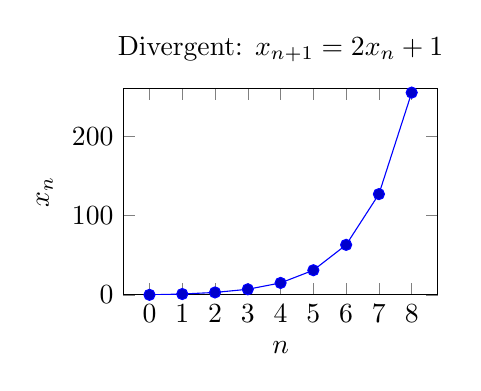
\begin{tikzpicture}
		\begin{axis}[
			width=0.46\textwidth,
			height=4.2cm,
			xlabel={$n$},
			ylabel={$x_n$},
			title={Divergent: $x_{n+1}=2x_n+1$},
			ymin=0, ymax=260,
			xtick={0,1,2,3,4,5,6,7,8}
			]
			\addplot+[mark=*] coordinates {
				(0,0)
				(1,1)
				(2,3)
				(3,7)
				(4,15)
				(5,31)
				(6,63)
				(7,127)
				(8,255)
			};
		\end{axis}
	\end{tikzpicture}
	
\end{figure}
\begin{DidacticBox}[Stabil vs.\ chaotisch: nicht verwechseln]
	\index{Chaos}
	Stabilität bedeutet nicht „langweilig“, und Instabilität bedeutet nicht automatisch „Zufall“.
	Auch chaotische Bahnen sind deterministisch, aber sie sind empfindlich gegenüber kleinsten Änderungen.
	Für unsere Zwecke reicht zunächst eine robustere Leitidee:
	\emph{beschränkt} versus \emph{unbeschränkt}.
	Der Grenzbereich zwischen beidem ist später der Ort der sichtbaren Struktur.
\end{DidacticBox}

\subsubsection*{Beschränktheit als Kriterium}
In der komplexen Ebene ist es besonders natürlich, den \emph{Betrag} $|z_n|$ zu betrachten.
Wir nennen einen Orbit \emph{beschränkt}, wenn es eine Zahl $R>0$ gibt, so dass
\[
|z_n|\le R \quad \text{für alle } n.
\]
Existiert kein solches $R$, dann läuft der Orbit ins Unendliche: $|z_n|\to\infty$.

\begin{MathBox}[Beschränkt oder unbeschränkt]
	\index{Beschränktheit}
	\index{Betrag}
	Für die Iteration $z_{n+1}=f(z_n)$ heißt der Orbit von $z_0$ \emph{beschränkt}, wenn
	\[
	\exists\, R>0:\ \forall n\in\mathbb{N}\ \ |z_n|\le R.
	\]
	Ist das nicht der Fall, nennt man den Orbit \emph{unbeschränkt} (oder divergent);
	typisch ist dann $|z_n|\to\infty$.
\end{MathBox}
\subsubsection*{Ein einfaches komplexes Beispiel: Spiralbahn im Kreis}
Wir betrachten die Iteration
\[
z_{n+1}=a\,z_n,\qquad a=0{,}85\,e^{i\pi/5},\qquad z_0=2+i.
\]
Da $|a|=0{,}85<1$ gilt
\[
|z_n|=|a|^n|z_0|\le |z_0|=:R=\sqrt{5}.
\]
Der Orbit bleibt also für alle $n$ im Kreisradius $R$ und spiralt gegen $0$.

\begin{figure}[h]
	\centering
	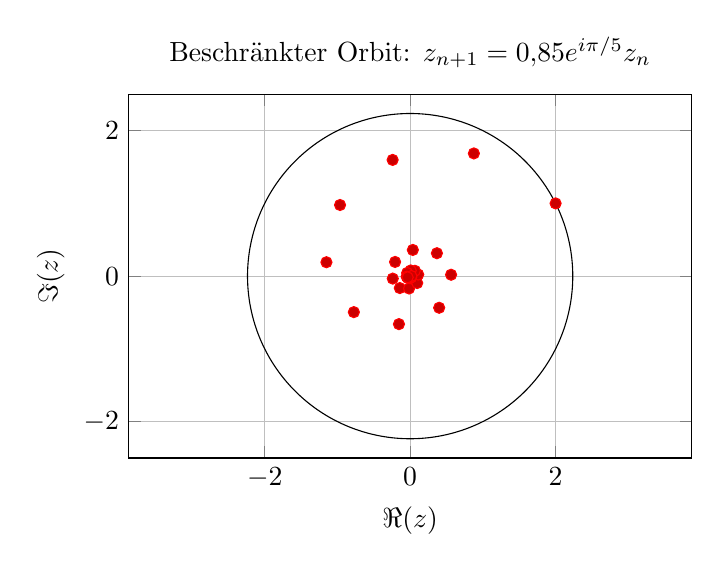
\begin{tikzpicture}
		\begin{axis}[
			axis equal,
			width=0.72\textwidth,
			height=6.2cm,
			xlabel={$\Re(z)$},
			ylabel={$\Im(z)$},
			title={Beschränkter Orbit: $z_{n+1}=0{,}85e^{i\pi/5}z_n$},
			xmin=-2.5, xmax=2.5,
			ymin=-2.5, ymax=2.5,
			grid=both
			]
			% Kreisradius R = sqrt(5)
			\addplot[domain=0:360, samples=361] ({sqrt(5)*cos(x)},{sqrt(5)*sin(x)});
			
			% Orbitpunkte (n=0..25)
			\addplot+[only marks, mark=*] coordinates {
				(2.000,1.000)
				(0.876,1.687)
				(-0.241,1.598)
				(-0.964,0.978)
				(-1.151,0.191)
				(-0.774,-0.495)
				(-0.154,-0.660)
				(0.399,-0.435)
				(0.563,0.019)
				(0.368,0.315)
				(0.037,0.360)
				(-0.207,0.195)
				(-0.239,-0.034)
				(-0.142,-0.164)
				(-0.015,-0.170)
				(0.097,-0.095)
				(0.111,0.022)
				(0.066,0.073)
				(0.008,0.078)
				(-0.041,0.044)
				(-0.048,-0.007)
				(-0.030,-0.026)
				(-0.005,-0.028)
				(0.015,-0.016)
				(0.017,0.002)
				(-0.034,-0.017)
			};
		\end{axis}
	\end{tikzpicture}
\end{figure}
\subsubsection*{Der Grenzfall: die eigentliche Bühne der Struktur}
Jetzt kommt der entscheidende Punkt für das ganze Kapitel:
Zwischen eindeutig stabil und eindeutig divergent liegt ein Randbereich, der extrem empfindlich ist.
Startwerte, die nur minimal voneinander abweichen, können völlig verschieden enden:
Der eine Orbit bleibt beschränkt, der andere fliegt weg.
Dieser „Übergang“ ist kein Nebeneffekt, sondern das Zentrum des Phänomens.

Genau deshalb entstehen später scharfe, fransige Grenzen und scheinbar unendliche Detailtiefe.
Nicht weil wir Natur modellieren, sondern weil wir eine mathematische Grenzfrage stellen.
\subsubsection*{Grenzfall: eine minimale Änderung entscheidet alles}
Wir betrachten die Iteration
\[
z_{n+1}=z_n^2,
\]
also die Quadratik $f(z)=z^2$. Hier lässt sich der Grenzfall vollständig verstehen:
\emph{Die Grenze zwischen beschränkt und unbeschränkt ist der Einheitskreis $|z|=1$.}
Damit ist bereits sichtbar, was später bei Mandelbrot- und Julia-Mengen in viel komplizierterer Form auftritt:
Ein Randbereich entscheidet über „bleibt drin“ oder „fliegt weg“.

Wir wählen zwei fast identische Startwerte:
\[
z_0=0{,}99 \quad (\text{knapp innerhalb}), 
\qquad z_0=1{,}01 \quad (\text{knapp außerhalb}).
\]

\begin{figure}[h]
	\centering
	
	% --- Bild links: komplexe Ebene mit Einheitskreis und Startpunkten ---
	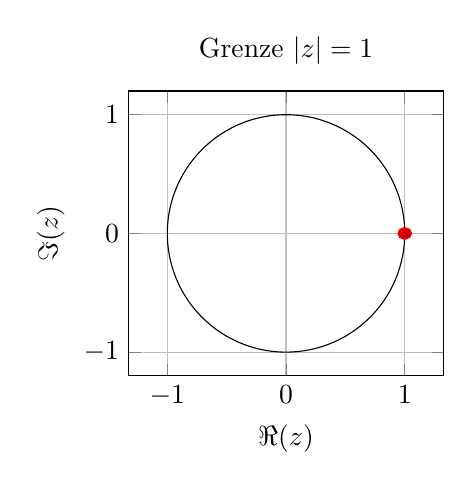
\begin{tikzpicture}
		\begin{axis}[
			axis equal,
			width=0.46\textwidth,
			height=5.2cm,
			xlabel={$\Re(z)$},
			ylabel={$\Im(z)$},
			title={Grenze $|z|=1$},
			xmin=-1.2, xmax=1.2,
			ymin=-1.2, ymax=1.2,
			grid=both
			]
			% Einheitskreis
			\addplot[domain=0:360, samples=361] ({cos(x)},{sin(x)});
			% Startpunkte
			\addplot+[only marks, mark=*] coordinates {(0.99,0) (1.01,0)};
		\end{axis}
	\end{tikzpicture}
	\hfill
	% --- Bild rechts: Betrag als Funktion von n (log-Skala) ---
	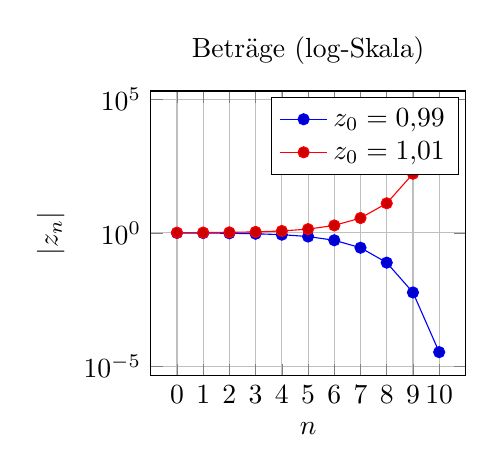
\begin{tikzpicture}
		\begin{axis}[
			width=0.46\textwidth,
			height=5.2cm,
			xlabel={$n$},
			ylabel={$|z_n|$},
			title={Beträge (log-Skala)},
			ymode=log,
			log basis y={10},
			xtick={0,1,2,3,4,5,6,7,8,9,10},
			grid=both
			]
			% z0=0.99
			\addplot+[mark=*] coordinates {
				(0,0.99)
				(1,0.9801)
				(2,0.96059601)
				(3,0.9227446944)
				(4,0.8514577711)
				(5,0.7249803360)
				(6,0.5255964875)
				(7,0.2762516677)
				(8,0.0763149839)
				(9,0.0058239768)
				(10,0.0000339187)
			};
			\addlegendentry{$z_0=0{,}99$}
			
			% z0=1.01
			\addplot+[mark=*] coordinates {
				(0,1.01)
				(1,1.0201)
				(2,1.04060401)
				(3,1.0828567056)
				(4,1.1725786449)
				(5,1.3749406785)
				(6,1.8904618695)
				(7,3.5738460800)
				(8,12.7723758032)
				(9,163.1335836586)
				(10,26612.5661173053)
			};
			\addlegendentry{$z_0=1{,}01$}
		\end{axis}
	\end{tikzpicture}
	
	\caption{Grenzfall bei $z_{n+1}=z_n^2$: Innerhalb des Einheitskreises bleiben Bahnen beschränkt, außerhalb divergieren sie. Schon eine minimale Änderung des Startwerts kann das Verhalten vollständig kippen.}
\end{figure}
\subsubsection*{Vorbereitung auf die Quadratik $z^2+c$}
\index{Quadratische Abbildung}
Für die Familie $f_c(z)=z^2+c$ wird es sogar ein praktisches Kriterium geben:
Wenn der Betrag eines Orbit irgendwann groß genug wird, dann ist sicher, dass er weiter wächst und entkommt.
Damit lässt sich „dazugehörig“ versus „nicht dazuzugehörig“ rechnerisch entscheiden.

\noindent\textbf{Übergang:} Im nächsten Abschnitt verwenden wir genau diese Idee als Landkarte:
Für welche Parameter $c$ bleibt der Orbit von $z_0=0$ beschränkt?
Die Antwort ist die Mandelbrot-Menge.






\subsection{Die Mandelbrot-Menge als Landkarte}
Kant

\subsection{Julia-Mengen: lokale Dynamik und Struktur}
Heu
\subsection{Selbstähnlichkeit und Skaleninvarianz}
He

\subsection{Warum diese Formen keine Naturmodelle sind}
Heute

\subsection{	Fazit: Struktur ohne Materie}
Heut
	\chapter{Mathematik und Philosophie}
\label{chap:VIII_philosophie}






% ================================
% Teil III – Mathematik und Philosophie
% ================================

%8.1
\subsection{Platon und die Ideenwelt}\label{sec:8.1}
\index{Platon}
\index{Ideenwelt}
\index{Platonismus}
\index{Entdeckung vs. Erfindung}
\index{Mathematische Objektivität}

\textbf{Leitfrage:} Ist Mathematik erfunden oder entdeckt?

\medskip
Wer sich ernsthaft mit Mathematik beschäftigt, stößt früher oder später auf eine merkwürdige Erfahrung:
Mathematische Aussagen wirken nicht wie menschliche Vereinbarungen, sondern wie \emph{Notwendigkeiten}.
Man kann sie formulieren, diskutieren, beweisen oder widerlegen -- aber man kann sie nicht per Beschluss ändern.
Genau an dieser Stelle ist Platon bis heute der klassische Bezugspunkt.

\subsubsection*{Zwei Ebenen: Sinnenwelt und Ideenwelt}
Platon unterscheidet zwischen zwei Bereichen.
In der \emph{Sinnenwelt} erleben wir konkrete Dinge: ungenaue Formen, wechselnde Zustände, Messfehler, Materialgrenzen.
Ein gezeichneter Kreis ist nie perfekt, eine gerade Linie hat immer eine Breite, ein Dreieck auf Papier ist immer leicht verzogen.
Dem stellt Platon die \emph{Ideenwelt} gegenüber:
Sie enthält die idealen Formen, die unveränderlichen Begriffe und die reinen Strukturen.
Dort ist der Kreis exakt, die Gerade hat keine Dicke, und das Dreieck besitzt genau die Eigenschaften, die seine Definition verlangt.
\newpage
\noindent
\begin{HistoryBox}[Platon: Mathematik als Zugang zur Ideenwelt]
	\small
	Platon (ca.\ 428--348 v.\,Chr.) vertrat die Auffassung, dass hinter den wandelbaren Dingen der Sinnenwelt
	eine Ebene idealer, unveränderlicher Formen (``Ideen'') steht.
	Mathematik gilt in diesem Denken als besonders geeignet, weil sie nicht von Messungen abhängt,
	sondern von Definitionen und logischer Notwendigkeit.
\end{HistoryBox}

\subsubsection*{Warum Mathematik objektiv wirkt}
Platons Argument ist im Kern einfach:
Mathematik beschreibt nicht das Unperfekte, sondern das Ideale.
Eine physikalische Messung liefert Näherungen.
Ein mathematischer Satz dagegen ist entweder wahr oder falsch -- unabhängig davon, ob wir ihn schon kennen.
Diese Unabhängigkeit erzeugt den Eindruck, dass mathematische Strukturen \emph{entdeckt} werden.

Ein Beispiel macht das sofort greifbar:
Ein Kreis aus Metall kann minimal oval sein, der Stiftstrich hat Dicke, das Papier wellt sich.
Der mathematische Kreis ist davon völlig unabhängig.
Er ist keine materielle Sache, sondern eine definierte Struktur:
die Menge aller Punkte mit konstantem Abstand \(r\) vom Mittelpunkt.
Gerade weil diese Definition unabhängig von jeder konkreten Zeichnung ist,
kann Mathematik mit einer Strenge arbeiten, die in der Naturbeobachtung so nicht möglich ist.
\newpage
\noindent
\subsubsection*{Entdecken statt Erfinden: ein Zahlenbeispiel}
Noch klarer wird es bei Zahlen.
Ob eine Zahl prim ist, hängt nicht von unserer Meinung ab.
Die Eigenschaft ``prim'' ist eine strukturierte Aussage über Teilbarkeit.
Wir können andere Symbole verwenden, andere Zahlensysteme oder andere Sprachen --
aber die Tatsache bleibt dieselbe.

\begin{DidacticBox}[Entdecken vs.\ Erfinden]
	\small
	Wir \emph{erfinden} Notationen (Symbole, Schreibweisen, Zahlensysteme).
	Aber wir \emph{entdecken} Beziehungen, die aus den Definitionen folgen:
	Teilbarkeit, Primzahlstruktur, logische Konsequenzen.
	Der Unterschied ist zentral: Die Form der Darstellung ist menschlich,
	die zugrunde liegende Struktur wirkt objektiv.
\end{DidacticBox}

Ein klassisches Beispiel für diese Objektivität ist ein Beweis:
Euklids Argument, dass es unendlich viele Primzahlen gibt, ist nicht empirisch, sondern zwingend.
Ein solcher Beweis ist kein ``Experiment'', sondern eine logische Notwendigkeit.
Gerade das passt zu Platons Idee: Mathematik besitzt eine Gültigkeit, die nicht von Beobachtung abhängt.

\subsubsection*{Platonismus heute: eine Deutung, kein Dogma}
In der modernen Philosophie der Mathematik nennt man die platonische Grundhaltung oft \emph{Mathematical Platonism}:
Mathematische Objekte gelten als unabhängig von uns.
Das ist keine naturwissenschaftliche These, die man im Labor messen könnte,
sondern eine Interpretation, warum Mathematik so zwingend und kulturübergreifend funktioniert.

\begin{NoteBox}[Wichtig: kein naiver ``Himmel der Zahlen'']
	\small
	Platonismus muss nicht bedeuten, dass Zahlen ``irgendwo im Raum'' existieren.
	Die Kernidee ist nüchterner: Mathematische Wahrheiten hängen nicht an Material,
	nicht an Kultur und nicht an Willkür -- sie folgen aus Struktur.
\end{NoteBox}
\newpage
\noindent
\subsubsection*{Übergang}
Platon erklärt, warum Mathematik so objektiv und zwingend wirkt.
Aber damit ist die zweite Frage noch offen:
Wie kommt diese ideale Strenge in die Praxis -- in Messen, Bauen, Rechnen, Naturwissenschaft?
Genau hier setzt Aristoteles an: Mathematik als Abstraktion aus der Erfahrung.




%8.2

\subsection{Aristoteles und die praktische Mathematik}\label{sec:8.2}
\index{Aristoteles}
\index{Abstraktion}
\index{Modell}
\index{Idealisierung}
\index{Grenzbegriff}

\textbf{Leitfrage:} Wenn Mathematik so ``ideal'' ist -- warum funktioniert sie dann in der Praxis und in den Wissenschaften?

\medskip
Nach Platon steht Mathematik in enger Beziehung zur Ideenwelt: Sie beschreibt ideale Strukturen, die nicht von Materie abhängen.
Aristoteles setzt den Schwerpunkt anders.
Er akzeptiert zwar die Strenge der Mathematik, aber er verortet sie näher an der Erfahrungswelt:
Mathematische Begriffe entstehen nicht in einem separaten ``Reich der Ideen'', sondern durch \emph{Abstraktion} aus dem Beobachtbaren.

\subsubsection*{Abstraktion statt Ideenwelt}
Aristoteles unterscheidet zwischen Dingen, die \emph{in der Natur} vorkommen, und Eigenschaften, die wir gedanklich \emph{isolieren}.
Wir sehen keine perfekten Geraden oder Kreise.
Aber wir können aus realen Formen das Wesentliche herauslösen:
Länge ohne Breite, Richtung ohne Material, Verhältnis ohne Stoff.
Mathematik ist in diesem Sinn kein Blick in eine eigene Welt, sondern ein Verfahren:
\emph{Wir abstrahieren von der Materie und behalten Struktur.}

\begin{HistoryBox}[Aristoteles: Mathematik als Abstraktion]
	\small
	Aristoteles (384--322 v.\,Chr.) betont, dass mathematische Gegenstände nicht als getrennte Dinge existieren,
	sondern durch Abstraktion aus der Erfahrungswelt gewonnen werden.
	Die Mathematik betrachtet Formen, Größen und Relationen, indem sie von Stoff, Zweck und Veränderung absieht.
\end{HistoryBox}

\subsubsection*{Warum ``praktische'' Mathematik funktioniert}
Damit wird verständlich, warum Mathematik so zuverlässig in Technik und Naturwissenschaft wirkt:
Sie trifft nicht die Materie direkt, sondern die \emph{Form} der Zusammenhänge.
Ein Ingenieur interessiert sich im ersten Schritt nicht für jedes Atom eines Balkens,
sondern für die Strukturgrößen, die das Verhalten dominieren: Länge, Querschnitt, Elastizität, Last.
Das ist aristotelisch gedacht:
Man entfernt Details, bis das Modell gerade so einfach ist, dass es rechenbar wird -- und gerade so reich, dass es die Wirklichkeit trifft.

\begin{DidacticBox}[Mathematik in der Praxis: richtiges Weglassen]
	\small
	Praktische Mathematik ist nicht ``unexakt'', sondern \emph{gezielt}.
	Sie lässt Details weg, die für die Frage unwesentlich sind,
	und behält jene Struktur, die das Verhalten dominiert.
	Gute Modelle sind keine perfekten Kopien der Welt, sondern präzise Abstraktionen.
\end{DidacticBox}

\subsubsection*{Platon vs.\ Aristoteles: der Unterschied in einem Satz}
Platon erklärt die Objektivität der Mathematik durch eine eigenständige Ebene idealer Strukturen.
Aristoteles erklärt die Anwendbarkeit der Mathematik durch Abstraktion aus der Erfahrung.
Beide Perspektiven sind kompatibel mit der täglichen mathematischen Praxis, aber sie betonen unterschiedliche Punkte:

\begin{itemize}
	\item \textbf{Platonisch:} Mathematik ist unabhängig von der Welt -- und trifft sie dennoch.
	\item \textbf{Aristotelisch:} Mathematik entsteht aus der Welt durch Abstraktion -- und ist deshalb anwendbar.
\end{itemize}

\subsubsection*{Ein kurzes Beispiel: die Gerade}
Eine reale Kante ist nie unendlich dünn, nie vollkommen glatt, nie exakt gerade.
Trotzdem ist das Konzept der Geraden in der Praxis extrem wirksam:
Es genügt, die Abweichungen als Toleranzen zu behandeln.
Die Gerade ist dann nicht ``eine Sache'', sondern ein Grenzbegriff,
an dem reale Objekte gemessen und verbessert werden.
\newpage
\noindent
\begin{NoteBox}[Grenzbegriffe in der Modellbildung]
	\small
	Viele mathematische Objekte sind Grenzbegriffe:
	punktförmige Massen, reibungsfreie Lager, ideale Geraden, perfekte Kreise.
	Sie existieren nicht als Dinge, aber sie sind als \emph{Struktur-Referenzen} unverzichtbar,
	weil sie das Rechnen ermöglichen und Abweichungen messbar machen.
\end{NoteBox}

\subsubsection*{Übergang zu Kant}
Platon verortet mathematische Wahrheit in einer eigenständigen Welt idealer Strukturen.
Aristoteles erklärt ihre Anwendbarkeit durch Abstraktion aus der Erfahrung.
Beide Positionen lassen jedoch eine dritte Möglichkeit offen, die Kant radikal formuliert:

\medskip
\noindent\emph{Was, wenn Mathematik weder ``dort draußen'' noch aus der Erfahrung stammt,
	sondern eine Bedingung dafür ist, dass Erfahrung überhaupt möglich wird?}

\medskip
Damit verschiebt sich die Leitfrage von der Ontologie zur Erkenntnistheorie:
Nicht nur \emph{was} Mathematik ist, sondern \emph{wie} sie in unserem Erkennen wirkt.
Und genau hier setzt Kant an.
%8.3
\subsection{Kant und die Bedingungen der Erkenntnis}\label{sec:8.3}
\index{Kant, Immanuel}
\index{Erkenntnistheorie}
\index{Raum und Zeit}
\index{synthetisch a priori}
\index{Ding an sich}

\textbf{Leitfrage:} Liegt Mathematik in der Welt -- oder liegt sie in uns?

\medskip
Platon verortet mathematische Wahrheit in einer eigenständigen Ideenwelt.
Aristoteles erklärt Mathematik als Abstraktion aus der Erfahrung.
Immanuel Kant setzt an einer anderen Stelle an: nicht bei der Frage, \emph{wo} mathematische Objekte existieren,
sondern bei der Frage, \emph{wie} Erkenntnis überhaupt möglich ist.
Damit verschiebt sich der Fokus von der Ontologie zur Erkenntnistheorie.

\subsubsection*{Kants Ausgangspunkt: Erfahrung braucht Form}
Kant beobachtet ein Problem, das bis heute zentral ist:
Aus bloßer Erfahrung allein erhält man niemals strenge Notwendigkeit.
Erfahrung zeigt, \emph{wie} etwas ist, aber nicht, dass es \emph{nicht anders sein kann}.
Mathematische Sätze wirken jedoch notwendig und allgemein gültig.
Also stellt Kant die entscheidende Frage:
Wie kann es Erkenntnisse geben, die notwendig sind, ohne bloß Definitionen zu sein?

\begin{HistoryBox}[Immanuel Kant und die ``Kritik der reinen Vernunft'']
	\small
	Immanuel Kant (1724--1804) untersuchte in der \emph{Kritik der reinen Vernunft} die Bedingungen der Möglichkeit von Erkenntnis.
	Berühmt ist seine These, dass Raum und Zeit nicht einfach Eigenschaften der Dinge ``an sich'' sind,
	sondern Formen unserer Anschauung: Wir erleben die Welt notwendig räumlich und zeitlich.
\end{HistoryBox}

\subsubsection*{Raum und Zeit als Formen der Anschauung}
Kants Kernidee ist radikal und zugleich praktisch verständlich:
Wir nehmen die Welt nicht roh auf, sondern immer durch grundlegende Strukturen, die unser Erkennen bereitstellt.
Dazu zählen insbesondere \emph{Raum} und \emph{Zeit}.
Sie sind in diesem Denken nicht zuerst Eigenschaften der Außenwelt,
sondern Bedingungen dafür, dass uns überhaupt etwas als geordnetes Erlebnis erscheint.

Damit erklärt sich, warum Geometrie (als Mathematik des Raums) und Arithmetik (als Mathematik der Abfolge) so fundamental sind:
Sie beschreiben nicht nur die Welt, sondern die Formen, \emph{in denen} die Welt für uns erscheinen muss.

\begin{DidacticBox}[Kants Drehung der Frage]
	\small
	Platon fragt: \emph{Wo} sind die mathematischen Formen?
	Aristoteles fragt: \emph{Wie} abstrahieren wir sie aus der Erfahrung?
	Kant fragt: \emph{Welche Strukturen müssen bereits vorhanden sein, damit Erfahrung überhaupt möglich ist?}
\end{DidacticBox}

\subsubsection*{``Synthetisch a priori'': Mathematik als notwendige Erkenntnis}
Kant nennt mathematische Urteile \emph{synthetetisch a priori}:
\begin{itemize}
	\item \emph{a priori}, weil sie nicht aus Erfahrung stammen und dennoch notwendig gelten,
	\item \emph{synthtetisch}, weil sie den Inhalt unseres Wissens erweitern und nicht bloß Begriffe umformulieren.
\end{itemize}
Der Gedanke dahinter: Mathematik ist nicht nur ein Sprachspiel.
Sie hat Inhalt, aber dieser Inhalt beruht auf den Bedingungen unserer Erkenntnis.

Man kann das an einem einfachen Kontrast sehen:
``Alle Junggesellen sind unverheiratet'' ist zwar notwendig, aber es steckt nur im Begriff.
Ein geometrischer Satz dagegen (z.\,B.\ über Dreiecke) ist notwendig und zugleich informativ.
Kant behauptet: Diese Informativität ist möglich, weil wir Raum und Zeit bereits als Struktur mitbringen.

\subsubsection*{Was Kant gewinnt -- und was offen bleibt}
Kant liefert eine starke Erklärung dafür, warum Mathematik in der Wissenschaft so zuverlässig ist:
Wenn Raum und Zeit Bedingungen unseres Erkennens sind, dann ist Mathematik die Grammatik,
in der uns Erfahrung überhaupt erscheinen kann.

Gleichzeitig bleibt eine Spannung, die man klar benennen sollte:
Wenn Mathematik an unsere Erkenntnisbedingungen gebunden ist --
beschreibt sie dann die Welt selbst oder nur die Welt, \emph{wie sie uns erscheint}?
Kant unterscheidet hier zwischen dem \emph{Ding an sich} und der \emph{Erscheinung}.
Naturwissenschaft betrifft in seinem Rahmen die Erscheinungswelt, nicht das Ding an sich.

\begin{NoteBox}[Der Preis der Erklärung]
	\small
	Kant erklärt die Notwendigkeit der Mathematik, indem er sie an die Bedingungen unserer Erfahrung bindet.
	Damit stellt sich aber die Frage: Gilt Mathematik objektiv ``da draußen'' --
	oder gilt sie notwendig nur für die Welt, wie sie uns erscheint?
\end{NoteBox}

\subsubsection*{Übergang zu modernen Positionen}
Mit Kant ist die Triade komplett:
Platon betont die Unabhängigkeit der Mathematik,
Aristoteles ihre Abstraktion aus der Erfahrung,
Kant ihre Rolle als Bedingung der Möglichkeit von Erfahrung.
Moderne Positionen bewegen sich bis heute in diesem Spannungsfeld.
Sie präzisieren, verschieben oder kombinieren diese drei Pole -- vom Formalismus und Logizismus
bis zu konstruktiven und strukturalistischen Sichtweisen.

Für dieses Buch ist dabei nicht entscheidend, welches Etikett man wählt,
sondern welche Einsicht stabil bleibt: Mathematik beschreibt in erster Linie \emph{Strukturen}.
Und genau diese Strukturen tauchen in Naturwissenschaft und Technik wieder auf -- nicht als Stoff, sondern als Form von Ordnung.
%8.4
\subsection{Moderne Positionen}\label{sec:8.4}
\index{Philosophie der Mathematik}
\index{Formalismus}
\index{Logizismus}
\index{Konstruktivismus}
\index{Strukturalismus}
\index{Fiktionalismus}


\textbf{Leitfrage:} Was ist Mathematik aus heutiger Sicht -- Entdeckung, Erfindung, Sprache, Spiel oder Struktur?

\medskip
Nach Platon (Ideenwelt), Aristoteles (Abstraktion) und Kant (Erkenntnisbedingungen) ist die Bühne klar:
Moderne Positionen sind meist Varianten, Mischformen oder Präzisierungen dieser drei Pole.
Statt einer einzigen ``richtigen'' Antwort gibt es heute mehrere konsistente Deutungen,
die jeweils unterschiedliche Aspekte der Mathematik erklären -- und jeweils einen Preis haben.

\subsubsection*{Platonismus: Mathematik wird entdeckt}
Der moderne \emph{Platonismus} behauptet: Mathematische Objekte existieren unabhängig von uns.
Wir finden sie, wie man eine Landschaft kartiert.
Das erklärt sehr gut, warum Mathematik objektiv wirkt und kulturübergreifend funktioniert.
Der Preis: Man muss akzeptieren, dass es ``mathematische Gegenstände'' gibt, die nicht materiell sind.

\subsubsection*{Formalismus: Mathematik als Regelspiel}
Im \emph{Formalismus} ist Mathematik ein System von Symbolen und Umformungsregeln:
Axiome, Beweisregeln, Ableitungen.
Wahr ist, was im System korrekt herleitbar ist.
Das erklärt die technische Seite der Mathematik (Beweisen als kontrolliertes Verfahren) hervorragend.
Der Preis: Es erklärt nur schwer, warum Mathematik die Physik so präzise trifft -- denn ein Regelspiel könnte auch beliebig bleiben.

\subsubsection*{Logizismus: Mathematik als Teil der Logik}
Der \emph{Logizismus} (klassisch: Frege, Russell) versucht, Mathematik auf Logik zurückzuführen:
Mathematik wäre dann letztlich eine Fortsetzung logischen Schließens.
Das erklärt, warum Beweise so zwingend sind.
Der Preis: In der Umsetzung ist es kompliziert (Paradoxien, Axiomatisierung), und nicht jede Mathematik lässt sich elegant ``reduzieren''.

\subsubsection*{Intuitionismus und Konstruktivismus: Mathematik als Machbarkeit}
Der \emph{Intuitionismus} (und verwandte konstruktive Richtungen) akzeptiert nur Objekte,
die man konstruieren kann, und Beweise, die tatsächlich ein Verfahren liefern.
Hier wird Mathematik eng an ``Wissen durch Konstruktion'' gebunden.
Das ist extrem sauber für Algorithmik und Beweisinhalt.
Der Preis: Man muss auf Teile der klassischen Mathematik verzichten (z.\,B. bestimmte Existenzbeweise ohne Konstruktion).

\subsubsection*{Strukturalismus: Mathematik als Theorie von Beziehungen}
Eine besonders moderne und für dieses Buch zentrale Position ist der \emph{Strukturalismus}:
Mathematik handelt nicht primär von ``Dingen'', sondern von \emph{Strukturen} und \emph{Relationen}.
Die Natur der Objekte ist zweitrangig; entscheidend ist, wie sie zueinander stehen.
Zahlen sind dann nicht mystische Entitäten, sondern Positionen in einer Struktur (z.\,B. in den Peano-Axiomen),
und ein Raum ist durch seine Strukturgesetze bestimmt, nicht durch ein Material, aus dem er bestünde.

\begin{NoteBox}[Der strukturalistische Kern]
	\small
	Mathematik beschreibt keine Stoffe, sondern Beziehungen: Ordnung, Symmetrie, Invarianz, Transformation.
	Objekte sind in diesem Sinn \emph{Knoten} in einem Netz von Relationen.
	Das macht Mathematik zugleich abstrakt und erstaunlich universell.
\end{NoteBox}

\subsubsection*{Fiktionalismus und ``Als-ob'': Mathematik als nützliches Modellieren}
Der \emph{Fiktionalismus} betont: Wir sprechen über Zahlen, Funktionen oder unendliche Mengen
so, \emph{als ob} sie existieren -- weil es extrem nützlich ist.
Mathematik wäre dann ein hochoptimiertes Modellwerkzeug.
Das erklärt die Praxisnähe (``es funktioniert'') ohne metaphysische Verpflichtungen.
Der Preis: Die objektive Zwingendheit vieler Sätze wirkt dann wie ein Nebenprodukt des Regelapparats,
nicht wie eine Aussage über ``etwas Reales''.

\subsubsection*{Die Schlüsselfrage der Moderne: Warum passt Mathematik zur Physik?}
Hier kulminiert alles.
Dass Mathematik intern konsistent sein kann, erklären Formalismus und Logik gut.
Dass Mathematik objektiv wirkt, erklärt der Platonismus gut.
Dass Mathematik konstruierbar und algorithmisch sein kann, erklärt der Konstruktivismus gut.
Aber die härteste Frage bleibt:

\medskip
\begin{quote}
	\emph{Warum ist Mathematik so wirksam in der Beschreibung der Natur?}
\end{quote}
\medskip

Hier kommen moderne realistische Positionen ins Spiel, insbesondere \emph{strukturaler Realismus}:
Die Physik erkennt nicht notwendigerweise ``Dinge an sich'',
aber sie erkennt stabile \emph{Strukturen} der Welt (Symmetrien, Erhaltungssätze, Invarianten, Gesetzesformen).
Mathematik passt dann zur Natur, weil die Natur selbst in entscheidenden Aspekten \emph{strukturhaft} ist.

\begin{DidacticBox}[Klarer Satz ohne Mystik]
	\small
	Dass Mathematik funktioniert, ist kein Beweis für eine ``magische Ideenwelt''.
	Aber es ist ein starkes Indiz dafür, dass die Welt in ihrem Verhalten regelhaft, symmetrisch und invariant ist --
	also mathematische Struktur besitzt.
\end{DidacticBox}

\subsubsection*{Fazit: ein nüchterner Standpunkt}
Die Moderne liefert keine letzte Einheitslehre, aber eine klare Einsicht:
Mathematik ist zugleich
\begin{itemize}
	\item \emph{formal} (Regeln, Beweise, Axiome),
	\item \emph{praktisch} (Modellieren, Approximieren, Rechnen),
	\item \emph{und strukturell} (Relationen, Invarianten, Symmetrien).
\end{itemize}
Je nach Blickwinkel betont man eines davon stärker.
Für den roten Faden dieses Buchs ist die strukturelle Sicht entscheidend:
Mathematik ist nicht bloß ein Zeichensystem und nicht bloß eine Beobachtungssprache,
sondern eine präzise Theorie von Strukturen -- und genau diese Strukturen tauchen in Natur, Technik und Denken wieder auf.

\subsubsection*{Übergang}
Damit ist der philosophische Rahmen gesetzt:
Wir können Mathematik als entdeckte Struktur (platonisch), als Abstraktion (aristotelisch),
als Bedingung von Erfahrung (kantisch) und als formales System (modern) verstehen.
Im weiteren Verlauf zählt nun nicht mehr das Etikett, sondern die Konsequenz:
Wir nutzen Mathematik als Werkzeug -- und behalten gleichzeitig im Blick, \emph{was} sie uns über Struktur verrät.
\subsection{Fazit: Mathematik als Struktur zwischen Welt und Denken}\label{sec:8.5}
\index{Struktur}


\textbf{Leitfrage:} Was bleibt nach Platon, Aristoteles, Kant und den modernen Positionen?

\medskip
Dieses Kapitel hat vier Blickrichtungen auf dieselbe Sache gezeigt:
Platon betont die Unabhängigkeit mathematischer Wahrheiten,
Aristoteles ihre Herkunft aus Abstraktion,
Kant ihre Rolle als Bedingung der Möglichkeit von Erfahrung,
und die Moderne präzisiert diese Pole durch formale, konstruktive und strukturalistische Ansätze.

\medskip
Die gemeinsame Kernaussage lässt sich nüchtern formulieren:
Mathematik ist zugleich \emph{Regelwerk}, \emph{Abstraktion} und \emph{Struktur}.
Wir erfinden Zeichen, Definitionen und Notationen -- aber wir entdecken Konsequenzen,
die aus den Regeln folgen und nicht von Meinung, Kultur oder Zeit abhängen.

\begin{NoteBox}[Arbeitsdefinition für dieses Buch]
	\small
	Mathematik ist die Theorie von Strukturen:
	von Beziehungen, Invarianten, Symmetrien und Gesetzesformen.
	Gerade deshalb ist sie universell anwendbar -- nicht, weil sie ``magisch'' ist,
	sondern weil Welt und Erkenntnis in entscheidenden Aspekten strukturhaft sind.
\end{NoteBox}

Damit ist der philosophische Rahmen gesetzt, ohne in Spekulation abzugleiten:
Das Buch nutzt Mathematik als Werkzeug, aber es behält die Grundfrage im Blick,
was diese Werkzeughaftigkeit über die Welt verrät.
Denn wenn Mathematik so zuverlässig funktioniert, dann ist das mindestens ein Hinweis darauf,
dass die Wirklichkeit nicht beliebig ist, sondern eine objektive Struktur besitzt --
und genau diese Struktur ist das eigentliche Thema dieses Buchs.

	\chapter{Mathematik im 21. Jahrhundert}
\label{chap:VIII_21jh}
\label{chap:VII_philosophie}
\label{chap:VIII_ausblick}




\subsection{Gödel und die Grenzen formaler Systeme}
Mit seinen Unvollständigkeitssätzen zeigte \textbf{Gödel, Kurt}\index{Gödel, Kurt}, 
dass es in jedem formalen System wahre Aussagen gibt, die nicht beweisbar sind. 
Dies veränderte das Verständnis von Mathematik grundlegend. 

\subsection{Computer und künstliche Intelligenz}
Computer haben die Mathematik praktisch und theoretisch revolutioniert. 
Von automatisierten Beweisen bis hin zu \textbf{künstlicher Intelligenz}\index{Künstliche Intelligenz} 
stellt sich die Frage: Lösen Maschinen nur Aufgaben – oder entdecken sie selbst Strukturen? 

\subsection{Mathematik und moderne Physik}
Die heutige Physik – von der Relativitätstheorie bis zur Quantenfeldtheorie – 
zeigt, dass Mathematik nicht nur Werkzeug ist, sondern den Rahmen der Naturgesetze vorgibt. 

\subsection{Ausblick: Die Struktur der Welt}
Die Reise führt zu einer offenen Frage: 
Ist Mathematik die Sprache, die wir erfinden – oder die Struktur, die wir entdecken? 
Vielleicht ist sie beides zugleich: ein Spiegel des Geistes und der Welt. 

	% Anhänge
	
\cleardoublepage
\appendix
\renewcommand{\thechapter}{A}

\renewcommand{\thesection}{\Alph{chapter}.\arabic{section}}

\chapter{Mathematische Hintergründe und Herleitungen}
\label{anhangA}

In diesem Anhang werden die im Haupttext angesprochenen physikalischen Konzepte
formal und mathematisch vertieft. Ziel ist es, die didaktische Lesbarkeit der
Kapitel nicht zu beeinträchtigen und zugleich interessierten Lesern die
vollständigen Herleitungen zugänglich zu machen. 


%\section{Kapitel I}
\phantomsection
\section{Herleitung der Irrationalität der $\sqrt{2}$}
\label{anhangA_wurzel2}


\subsection*{Die Irrationalität von \texorpdfstring{$\sqrt{2}$}{sqrt(2)}}
\phantomsection

Der Beweis, dass $\sqrt{2}$ irrational ist, gehört zu den ältesten und
elegantesten Widerspruchsbeweisen \index{Widerspruchsbeweis}der Mathematik. 
Die Idee ist einfach: Wir nehmen an, dass $\sqrt{2}$ rational sei, und
zeigen dann, dass diese Annahme zu einem logischen Widerspruch führt.

\subsubsection*{Annahme}
\phantomsection
Wir nehmen an, dass $\sqrt{2}$ als vollständig gekürzter Bruch
\[
\sqrt{2} = \frac{p}{q},
\]
geschrieben werden kann, wobei $p$ und $q$ ganze Zahlen sind,
$q \neq 0$ und $p$ und $q$ teilerfremd sind.

\subsubsection*{Quadratbildung}
\phantomsection
Quadrieren beider Seiten ergibt
\[
2 = \frac{p^2}{q^2}
\qquad\Rightarrow\qquad
p^2 = 2q^2.
\]

Die rechte Seite ist gerade, also muss auch $p^2$ gerade sein.
Damit ist auch $p$ gerade. Es gibt also eine ganze Zahl $r$ mit
\[
p = 2r.
\]

\subsubsection*{Einsetzen und erneuter Schluss}
\phantomsection
Setzen wir dies in die Gleichung $p^2 = 2q^2$ ein, erhalten wir
\[
(2r)^2 = 2q^2,
\]
also
\[
4r^2 = 2q^2.
\]

Teilen durch $2$ liefert
\[
2r^2 = q^2.
\]

Also ist auch $q^2$ gerade – und damit $q$ selbst gerade.

\subsubsection*{Der Widerspruch}
\phantomsection
\index{Widerspruch}
Wir haben nun gezeigt:
\[
p \text{ ist gerade}, \qquad q \text{ ist gerade}.
\]
Damit besitzen $p$ und $q$ einen gemeinsamen Faktor $2$ und sind nicht
teilerfremd.

Das widerspricht unserer Ausgangsannahme, dass $\frac{p}{q}$ vollständig
gekürzt ist.

\subsubsection*{Folgerung}
Die Annahme, $\sqrt{2}$ sei rational, führt zum Widerspruch. Daher muss
\[
\sqrt{2} \text{ irrational sein.}
\]

Dieser klassische Beweis geht in seinen Grundzügen bereits auf Euklid\index{Euklid}
zurück und zeigt eindrucksvoll, wie Widerspruchsbeweise funktionieren.



\begin{DidacticBox}[Warum dieser Beweis so elegant ist]
	Der Beweis für die Irrationalität von $\sqrt{2}$ ist ein klassisches
	Beispiel dafür, wie mächtig Widerspruchsbeweise sein können. 
	Aus einer scheinbar harmlosen Annahme folgt eine logische Unmöglichkeit.
	Damit zeigt der Beweis nicht nur, dass $\sqrt{2}$ irrational ist, 
	sondern auch, wie präzise mathematisches Denken funktioniert.
\end{DidacticBox}




\section{Konstruktion der komplexen Zahlen}\index{komplexe Zahlen}
\label{anhangA_komplexe}
%\subsection*{A.2 Konstruktion der komplexen Zahl}
\phantomsection
\index{komplexe Zahlen}
Die Notwendigkeit komplexer Zahlen ergibt sich aus einem einfachen
Problem: Manche Gleichungen besitzen in den reellen Zahlen keine Lösung.
Das deutlichste Beispiel ist
\[
x^2 + 1 = 0.
\]

Durch Umformen erhält man
\[
x^2 = -1.
\]

Doch keine reelle Zahl besitzt ein negatives Quadrat. Damit zeigt sich
eine Grenze des reellen Zahlensystems. Trotzdem treten solche Ausdrücke
beim Lösen bestimmter Gleichungen – etwa im \emph{casus irreducibilis}\index{casus irreducibilis}
kubischer Gleichungen – zwangsläufig auf.

\subsubsection*{Ein neuer Zahlentyp}
\phantomsection
Um die Gleichung $x^2 = -1$ lösbar zu machen, führt man eine neue Zahl
ein und definiert
\[
i := \sqrt{-1}.
\]
\index{imaginäre Einheit $i$}
Diese Definition ist kein Trick, sondern eine Erweiterung des
Zahlensystems: Wir ergänzen die reellen Zahlen so, dass auch Gleichungen
mit negativen Quadraten sinnvoll lösbar werden.

\subsubsection*{Der Aufbau des neuen Zahlentyps}
\phantomsection
Jede Zahl der Form
\[
a + bi, \qquad a,b \in \mathbb{R},
\]
\index{komplexe Zahl $a+bi$}
heißt \emph{komplexe Zahl}. Die bekannten Rechenregeln bleiben gültig;
die einzige neue Information ist
\[
i^2 = -1.
\]

Daraus lassen sich Addition und Multiplikation vollständig bestimmen.
Ein Beispiel:
\[
(2 + 3i)(4 - i)
= 8 - 2i + 12i - 3i^2
= 11 + 10i.
\]

\begin{DidacticBox}[Warum die Einführung von $i$ notwendig ist]
	Die Zahl $i$ wird nicht eingeführt, weil man sie „erfinden“ wollte.
	Sie entsteht aus der inneren Logik der Algebra. Sobald man die
	Rechenregeln für Gleichungen akzeptiert, erzwingt die Gleichung
	$x^2 = -1$ die Einführung eines neuen Zahlentyps. 
	
	Alle komplexen Zahlen folgen dann aus der minimalen Annahme
	$i^2 = -1$. Damit wird das Zahlensystem abgeschlossen: Jedes Polynom
	besitzt nun mindestens eine Lösung (Fundamentalsatz der Algebra).\index{Fundamentalsatz der Algebra}
\end{DidacticBox}
\subsubsection*{Die Euler-Formel als geometrische Ergänzung}
\index{Euler-Formel}
\phantomsection
Die Einführung der Zahl $i$ erschließt nicht nur einen neuen Zahlenbereich,
sondern verbindet auch die Exponentialfunktion mit Kreisbewegungen.
Dies zeigt sich in der berühmten Euler-Formel
\[
e^{i\varphi} = \cos\varphi + i\sin\varphi.
\]
\subsubsection*{Kurze Herleitung der Euler-Formel mit Taylor-Reihen}
\phantomsection
\index{Taylor-Reihe}
Die Euler-Formel
\[
e^{i\varphi} = \cos\varphi + i\sin\varphi
\]
lässt sich elegant mit Potenzreihen (Taylor-Reihen) herleiten.

Zunächst betrachten wir die Reihenentwicklungen der Funktionen
$e^x$, $\cos x$ und $\sin x$ um den Punkt $x=0$:
\begin{align*}
	e^x &= 1 + x + \frac{x^2}{2!} + \frac{x^3}{3!} + \frac{x^4}{4!} + \cdots,\\[1ex]
	\cos x &= 1 - \frac{x^2}{2!} + \frac{x^4}{4!} - \frac{x^6}{6!} + \cdots,\\[1ex]
	\sin x &= x - \frac{x^3}{3!} + \frac{x^5}{5!} - \frac{x^7}{7!} + \cdots.
\end{align*}

Setzen wir nun in die Exponentialreihe $x = i\varphi$ ein, so erhalten wir
\[
e^{i\varphi} = 1 + i\varphi + \frac{(i\varphi)^2}{2!}
+ \frac{(i\varphi)^3}{3!}
+ \frac{(i\varphi)^4}{4!}
+ \cdots.
\]

Mit den Potenzen von $i$,
\[
i^2 = -1,\quad i^3 = -i,\quad i^4 = 1,\quad i^5 = i,\;\dots,
\]
können wir die Terme sortieren. Wir trennen Real- und Imaginärteil:

\begin{align*}
	e^{i\varphi}
	&= \Bigl(1 - \frac{\varphi^2}{2!} + \frac{\varphi^4}{4!} - \frac{\varphi^6}{6!} + \cdots\Bigr)
	\;+\; i\Bigl(\varphi - \frac{\varphi^3}{3!} + \frac{\varphi^5}{5!} - \frac{\varphi^7}{7!} + \cdots\Bigr)\\[1ex]
	&= \cos\varphi + i\sin\varphi.
\end{align*}

Damit ist die Euler-Formel
\[
e^{i\varphi} = \cos\varphi + i\sin\varphi
\]
als direkte Folge der Reihenentwicklungen von Exponential-, Sinus- 
und Kosinusfunktion hergeleitet.

\subsubsection*{Geometrische Idee}
\phantomsection
Betrachtet man die komplexe Ebene, so beschreibt ein Punkt auf dem
Einheitskreis \index{Einheitskreis} einen Winkel $\varphi$ zur reellen Achse.
Die Projektion auf die beiden Achsen ergibt
\[
(\cos\varphi,\;\sin\varphi).
\]
\index{Sinus}
\index{Kosinus}
Da die imaginäre Achse als Vielfaches von $i$ interpretiert wird,
entspricht dieser Punkt der komplexen Zahl
\[
\cos\varphi + i\sin\varphi.
\]

Die Euler-Formel zeigt, dass die komplexe Exponentialfunktion
genau diese Kreisbewegung beschreibt.

\begin{center}
	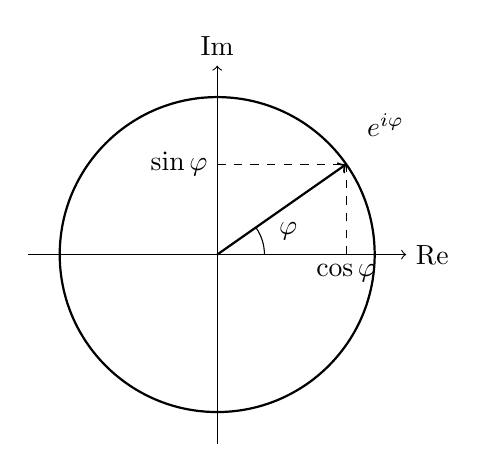
\begin{tikzpicture}[scale=2]
		% Kreis
		\draw[thick] (0,0) circle (1);
		% Achsen
		\draw[->] (-1.2,0) -- (1.2,0) node[right] {Re};
		\draw[->] (0,-1.2) -- (0,1.2) node[above] {Im};
		% Winkel
		\draw[thick,->] (0,0) -- ({cos(35)},{sin(35)});
		\draw (0.3,0) arc (0:35:0.3);
		\node at (0.45,0.15) {$\varphi$};
		% Projektionen
		\draw[dashed] ({cos(35)},0) -- ({cos(35)},{sin(35)});
		\draw[dashed] (0,{sin(35)}) -- ({cos(35)},{sin(35)});
		% Beschriftungen
		\node[below] at ({cos(35)},0) {$\cos\varphi$};
		\node[left] at (0,{sin(35)}) {$\sin\varphi$};
		\node at ({cos(35)+0.25},{sin(35)+0.25}) {$e^{i\varphi}$};
	\end{tikzpicture}
\end{center}

\subsubsection*{Multiplikation mit \boldmath$i$ als Drehung}
\phantomsection
\index{Drehung (Multiplikation mit $i$)}
In der komplexen Ebene hat die Multiplikation mit $i$ eine einfache geometrische 
Bedeutung: Sie dreht jede Zahl um $90^\circ$ gegen den Uhrzeigersinn.

Beispiele:
\[
1 \xrightarrow{\;\cdot i\;} i \xrightarrow{\;\cdot i\;} -1 
\xrightarrow{\;\cdot i\;} -i \xrightarrow{\;\cdot i\;} 1
\]

Jede weitere Multiplikation mit $i$ fügt eine weitere Drehung von $90^\circ$ hinzu.  
Wichtig: Die Länge (der Betrag) ändert sich dabei nicht – nur die Richtung.

Die Exponentialfunktion $e^{i\varphi}$ kombiniert unendlich viele solcher 
kleinen Drehungen. Dadurch entsteht eine kontinuierliche Rotation auf dem 
Einheitskreis, deren Winkel genau $\varphi$ beträgt.
\subsubsection*{Warum Multiplikation mit \boldmath$i$ eine Drehung erzeugt}
\phantomsection
Betrachten wir einen Punkt auf dem Einheitskreis:
\[
e^{i\varphi} = \cos\varphi + i\sin\varphi.
\]

Multiplizieren wir diesen Punkt mit $i$, so erhalten wir
\[
i \cdot e^{i\varphi}
= i(\cos\varphi + i\sin\varphi)
= i\cos\varphi - \sin\varphi.
\]

Dies entspricht der neuen komplexen Zahl
\[
-\sin\varphi + i\cos\varphi.
\]

Genau das erhält man auch, wenn man den ursprünglichen Punkt
\((\cos\varphi,\;\sin\varphi)\)
um \(90^\circ\) gegen den Uhrzeigersinn dreht:
\[
(\cos\varphi,\;\sin\varphi)
\;\longrightarrow\;
(-\sin\varphi,\;\cos\varphi).
\]

Damit ist klar:  
\[
i \cdot e^{i\varphi}
\]
ist \emph{genau} der Punkt, der um \(90^\circ\) gedreht wurde – bei unverändertem Radius.

\begin{DidacticBox}[Kernidee der Euler-Formel]
	Multiplikation mit $i$ bedeutet eine Drehung um $90^\circ$ in der komplexen Ebene.  
	Die Exponentialfunktion $e^{i\varphi}$ kombiniert viele solcher kleinen Drehungen 
	zu einer einzigen Rotation um den Winkel $\varphi$.
	
	Darum gilt:
	\[
	e^{i\varphi} = \cos\varphi + i\sin\varphi.
	\]
\end{DidacticBox}

\subsubsection*{Abschluss}
\phantomsection
Die komplexen Zahlen erweitern die reellen Zahlen um genau das, was
fehlt, um alle Gleichungen lösbar zu machen. Aus der einzelnen
Definition $i^2=-1$ entsteht ein vollständiger Zahlenbereich mit klaren
Regeln und einer geometrischen Struktur.
%============================================================
\section{Mandelbrot-Landkarte: mathematische Erzeugung und Farbgebung}
\label{app:mandelbrot-rendering}

\index{Mandelbrotmenge}
\index{Iteration}
\index{Escape-Radius}
\index{Fluchtzeit}
\index{Parameterraum}
\index{komplexe Ebene}
\index{Farbgebung}
\index{Algorithmus}

\textbf{Ziel dieses Anhangs:} Hier wird gezeigt, wie eine typische Mandelbrot-Grafik algorithmisch entsteht:
vom Bildpixel über den Parameter \(c\) bis zur Fluchtzeit und zur Farbzuordnung.

\begin{MathBox}[Grundprinzip: Pixel \(\rightarrow\) Parameter \(c\) \(\rightarrow\) Iteration]
	Wir berechnen für jeden Bildpunkt einen Parameter \(c\in\mathbb{C}\) und iterieren
	\[
	z_{n+1}=z_n^2+c,\qquad z_0=0.
	\]
	Die Mandelbrotmenge ist die Menge der Parameter \(c\), für die die Folge \(\{z_n\}\) beschränkt bleibt.
\end{MathBox}

%------------------------------------------------------------
\subsection*{Koordinatentransformation: vom Pixel in die komplexe Ebene}
\index{Koordinatentransformation}

Ein Bild habe Breite \(W\) und Höhe \(H\). Wir wählen ein Sichtfenster
\[
x\in[x_{\min},x_{\max}],\qquad y\in[y_{\min},y_{\max}]
\]
und ordnen jedem Pixel \((i,j)\) (mit \(0\le i<W\), \(0\le j<H\)) einen Parameter \(c=x+iy\) zu:
\[
x(i)=x_{\min}+\frac{i}{W-1}\,(x_{\max}-x_{\min}),\qquad
y(j)=y_{\max}-\frac{j}{H-1}\,(y_{\max}-y_{\min}),
\]
\[
c(i,j)=x(i)+i\,y(j).
\]
Das Minuszeichen bei \(y(j)\) kommt daher, dass Bildkoordinaten typischerweise nach unten wachsen.

\begin{NoteBox}[Typisches Standardfenster]
	Ein häufig verwendetes Fenster ist
	\[
	x\in[-2.5,1.0],\qquad y\in[-1.2,1.2].
	\]
	Für Details (Zoom) wählt man ein kleineres Fenster um ein Zentrum \(c_0\).
\end{NoteBox}

%------------------------------------------------------------
\subsection*{Escape-Time-Algorithmus: Fluchtkriterium und Iterationszahl}
\index{Fluchtkriterium}

Für jedes \(c\) iterieren wir bis zu einer Maximalzahl \(N_{\max}\). Sobald \(|z_n|>R\) gilt, stoppen wir.
Für die Mandelbrotiteration reicht klassisch \(R=2\):

\begin{MathBox}[Escape-Radius \(R=2\)]
	Für \(z_{n+1}=z_n^2+c\) gilt: Wenn für ein \(n\) \(|z_n|>2\), dann divergiert die Folge sicher.
\end{MathBox}

Formal definieren wir die \textbf{Fluchtzeit}
\[
n_\text{esc}(c)=\min\{n\in\mathbb{N}\mid |z_n|>2\},
\]
falls sie existiert; andernfalls setzen wir \(n_\text{esc}(c)=N_{\max}\) und markieren den Punkt als „innen“ (typisch schwarz).

%------------------------------------------------------------
\subsection*{Farbgebung: diskret, glatt und „schön“}
\index{Farbskala}

\subsubsection*{(a) Diskrete Farbgebung über Fluchtzeit}
Die einfachste Methode: ordne die Farbe nur nach \(n_\text{esc}\) zu.
Das führt oft zu sichtbaren „Bändern“ (Banding), ist aber didaktisch klar.

\subsubsection*{(b) Glatte Farbgebung (Continuous Coloring)}
Um Banding zu vermeiden, nutzt man eine \textbf{kontinuierliche} Iterationszahl. Eine verbreitete Variante ist:
\[
\nu(c)=n + 1 - \log_2\!\bigl(\log |z_n|\bigr),
\]
wobei \(n\) der erste Index ist mit \(|z_n|>2\). (Hier ist \(z_n\) bereits außerhalb; \(\nu\) liegt zwischen \(n\) und \(n+1\).)

\begin{DidacticBox}[Warum diese „Log-Log“-Formel?]
	Außerhalb wächst \(|z_n|\) ungefähr quadratisch. Durch \(\log(\log(\cdot))\) wird dieses Wachstum „linearisiert“,
	sodass Farbverläufe glatt werden und die Struktur am Rand deutlich besser sichtbar ist.
\end{DidacticBox}

Aus \(\nu\) macht man dann eine Zahl \(t\in[0,1]\) (z.B. durch Skalierung) und führt \(t\) durch eine Farbpalette.

\subsubsection*{(c) Histogramm-Equalization (optional, für sehr gleichmäßige Kontraste)}
Fortgeschritten: man zählt, wie viele Pixel welche Fluchtzeit haben, bildet eine kumulative Verteilung und verteilt Farben so,
dass häufige Werte nicht „zusammenkleben“. Das liefert sehr ausgewogene Bilder, ist aber reiner Rendering-Komfort.

%------------------------------------------------------------
\subsection*{Pseudocode: kompakt und nachvollziehbar}
\index{Pseudocode}

% Wenn du listings nutzt:
% \usepackage{listings}

\begin{verbatim}
	Input: W,H, x_min,x_max, y_min,y_max, N_max, R=2
	for j = 0..H-1:
	y = y_max - j*(y_max-y_min)/(H-1)
	for i = 0..W-1:
	x = x_min + i*(x_max-x_min)/(W-1)
	c = x + I*y
	z = 0
	n = 0
	while n < N_max and |z| <= R:
	z = z*z + c
	n = n + 1
	if n == N_max:
	color(i,j) = black   // inside (bounded up to N_max)
	else:
	// smooth iteration count (optional):
	nu = n + 1 - log2(log(|z|))
	color(i,j) = palette(nu)
	Output: PNG image
\end{verbatim}

\begin{NoteBox}[Wichtig für den Leser]
	Die Mandelbrotmenge selbst ist \emph{mathematisch} nur „innen vs. außen“ (beschränkt vs. divergent).
	Alles, was danach kommt (Palette, Glättung, Histogramm), ist \textbf{Darstellungstechnik}.
\end{NoteBox}

%============================================================
	\cleardoublepage
%\appendix
\renewcommand{\thechapter}{B}

\renewcommand{\thesection}{\Alph{chapter}.\arabic{section}}



\chapter{Boxenverzeichnis}
\label{anhangB}


%\chapter{Boxenverzeichnis}
\label{chap:boxenverzeichnis}
\thispagestyle{empty}


%\addcontentsline{toc}{chapter}{Anhang B – Boxenverzeichnis}


	\cleardoublepage

\renewcommand{\thesection}{\thechapter.\arabic{section}}
\renewcommand{\thechapter}{C}

\chapter{KI in der Wissenschaft – Werkzeug statt Wahrheit}
\phantomsection
\vspace{1em}
\begin{center}
	\LARGE\textbf{KI in der Wissenschaft – Werkzeug statt Wahrheit}
\end{center}

\subsection*{Motivation}
\phantomsection
Dieses Buch entstand aus dem Wunsch, die Grundlagen und Perspektiven der Quanteninformatik – vom Qubit über Algorithmen bis hin zu technischen Realisierungen – verständlich und fundiert darzustellen. 
Dabei wurde ein Werkzeug eingesetzt, das heute immer mehr Einzug in wissenschaftliches Arbeiten hält: \textbf{künstliche Intelligenz}\index{Künstliche Intelligenz}, konkret das Sprachmodell \textbf{ChatGPT}\index{ChatGPT} von OpenAI.

Doch wie lässt sich KI sinnvoll in der Wissenschaft\index{Wissenschaft} nutzen, ohne dass dabei Verständnis, Präzision oder Verantwortung\index{Verantwortung} verloren gehen? Und wie kann man das offenlegen, ohne die eigene wissenschaftliche Arbeit zu relativieren? Dieser Anhang gibt einen transparenten Einblick in den Entstehungsprozess dieses Buches und plädiert für einen verantwortungsvollen Umgang mit KI als Werkzeug – nicht als Wahrheit.

\subsection*{Was eine KI kann – und was nicht}
\phantomsection
KI-gestützte Sprachmodelle wie ChatGPT sind leistungsfähige Hilfsmittel beim Schreiben und Strukturieren. Sie können:
\begin{itemize}
	\item beim Formulieren erster Entwürfe helfen,
	\item komplexe Sachverhalte sprachlich glätten,
	\item Denkanstöße liefern oder Gliederungen vorschlagen,
	\item stilistische Alternativen aufzeigen.
\end{itemize}

Was sie jedoch \textbf{nicht} können:
\begin{itemize}
	\item \textbf{Verstehen}\index{Verstehen} im wissenschaftlichen Sinn,
	\item \textbf{prüfen}, ob eine mathematische Herleitung korrekt ist,
	\item \textbf{physikalische Konzepte oder Algorithmen durchdringen},
	\item \textbf{Quellen kritisch einordnen oder bewerten}.
\end{itemize}

Daher gilt: Eine KI kann \emph{unterstützen}, aber sie \textbf{kann und darf den wissenschaftlichen Erkenntnisprozess nicht ersetzen}. Wer mit KI arbeitet, muss dennoch selbst denken – und das Ergebnis stets kritisch prüfen.

\subsection*{Wie dieses Buch entstanden ist}
\phantomsection
Die Inhalte dieses Buches – von der Struktur über die physikalischen Erklärungen bis zu den mathematischen und algorithmischen Herleitungen – wurden vom Autor konzipiert, recherchiert und verantwortet. ChatGPT kam in folgenden Bereichen unterstützend zum Einsatz:

\begin{itemize}
	\item beim \textbf{Formulieren einzelner Passagen}, z.\,B. bei Einleitungen, Zusammenfassungen oder didaktischen Abschnitten,
	\item zur \textbf{Stilüberprüfung} technischer und algorithmischer Erklärungen,
	\item zur \textbf{Gliederungsentwicklung} in frühen Arbeitsphasen,
	\item zur Reflexion über \textbf{Verständlichkeit}\index{Verständlichkeit} und Leserführung.
\end{itemize}

Entscheidend ist: \textbf{Alle inhaltlichen Aussagen, Formeln, Algorithmen und Interpretationen wurden vom Autor geprüft, hinterfragt, überarbeitet oder verworfen.} Keine KI war an der inhaltlichen Entwicklung der physikalischen oder informatischen Argumentation beteiligt.

\subsection*{Ethische Fragen und wissenschaftliche Verantwortung}
\phantomsection
Die Nutzung von KI in der Wissenschaft wirft berechtigte Fragen auf:

\begin{itemize}
	\item Wie viel darf automatisiert entstehen, ohne dass Autorschaft\index{Autorschaft} verwässert?
	\item Wie geht man mit potenziellen Fehlern\index{Fehler} um?
	\item Wie transparent muss die Nutzung offengelegt werden?
\end{itemize}

Die Antwort liegt in einem Grundprinzip wissenschaftlicher Arbeit: \textbf{Verantwortung}. Wer KI einsetzt, bleibt verantwortlich für das Ergebnis – unabhängig davon, ob einzelne Formulierungen von einem Modell vorgeschlagen wurden.

In diesem Sinne ist KI keine Autorin, sondern ein Werkzeug. Sie kann Prozesse beschleunigen, aber nicht ersetzen, was Wissenschaft im Kern ausmacht: \textbf{kritisches Denken, sorgfältiges Prüfen, methodisches Arbeiten}.

\subsection*{Empfehlungen für den Einsatz in der Forschung}
\phantomsection
Für Wissenschaftler:innen, Lehrende und Studierende ergibt sich daraus ein konstruktiver Weg:

\begin{itemize}
	\item Nutze KI \textbf{bewusst und gezielt} – für sprachliche Unterstützung, nicht für Argumentation, Beweisführung oder Algorithmusentwicklung.
	\item \textbf{Prüfe jede Aussage selbst} – gerade bei komplexen Sachverhalten.
	\item \textbf{Deklariere die Nutzung offen}, wenn es relevant ist – z.\,B. in Vorworten, Anhängen oder Einreichungserklärungen.
	\item Nutze KI nicht zur \textbf{Täuschung}\index{Täuschung} oder zum Feigenblatt, sondern als Hilfe zur besseren Darstellung deiner eigenen Gedanken.
\end{itemize}

\subsection*{Fazit: KI als Werkzeug – aber der Mensch bleibt denkend verantwortlich}
\phantomsection
Künstliche Intelligenz ist weder Ersatz noch Gegner menschlicher Erkenntnis. Sie ist ein \textbf{Werkzeug}\index{Werkzeug}, das bei der wissenschaftlichen Kommunikation helfen kann – \textbf{wenn es bewusst, reflektiert und verantwortungsvoll eingesetzt wird}.

Dieses Buch versteht sich auch in dieser Hinsicht als Beitrag zu einem neuen, aufgeklärten Umgang mit Technologie in der Wissenschaft. Nicht, weil die Technik alles kann – sondern weil wir gelernt haben, sie sinnvoll zu nutzen.

\vspace{1em}
\begin{tcolorbox}[didaktikbox, title=Leitgedanke]
	\label{box:leitgedanke}
	\small
	\textbf{KI ist nur so stark, wie der Mensch, der sie benutzt.}\\
	Sie kann Texte strukturieren, formulieren, variieren – 
	doch ohne kritisches Denken, Fachwissen und Verantwortung 
	des Autors bleibt sie ein Werkzeug ohne Sinn.
\end{tcolorbox}

	
	% Literatur
	% Literaturverzeichnis ins Inhaltsverzeichnis aufnehmen
	\addcontentsline{toc}{chapter}{Literatur} % oder {Literatur} für Deutsch
	\printbibliography[title=Literatur]       % [title=Literatur] für Deutsch
	
	
	% Index
	\clearpage
	\phantomsection
	\addcontentsline{toc}{chapter}{Stichwortverzeichnis}
	\renewcommand{\indexname}{Stichwortverzeichnis}
	\cleardoublepage
	\printindex
	
	% Impressum (optional)
	% \chapter*{Impressum}
%\setcounter{section}{12}
%\setcounter{subsection}{0}
%\setcounter{subsubsection}{1}
%setcounter{secnumdepth}{3}
%\addcontentsline{toc}{chapter}{Impressum}
\label{chap:imp}
\begin{flushleft}
	
	\textbf{Titel:} \\
	Photon – Theorie und Anwendungen \\[1em]
	
	\textbf{Autor:} \\
	Christian Weilharter \\
	Dipl.-Ing. (FH) \\[1em]
	
	\textbf{Veröffentlichung:} \\
	Selbstverlag (Self-Publishing) oder Online-Publikation \\[1em]
	
	\textbf{Erscheinungsdatum:} \\
	8. Juni 2025 \\[1em]
	
	\textbf{Kontakt:} \\
	\[christian@weilharter.de\] \\[1em]
	
	\textbf{Urheberrecht:} \\
	Alle Rechte vorbehalten. Dieses Werk einschließlich aller seiner Teile ist urheberrechtlich geschützt. Jede Verwertung außerhalb der engen Grenzen des Urheberrechtsgesetzes ist ohne Zustimmung des Autors unzulässig. Dies gilt insbesondere für Vervielfältigungen, Übersetzungen, Mikroverfilmungen und die Einspeicherung und Verarbeitung in elektronischen Systemen. \\[1em]
	
	\textbf{Haftungsausschluss:} \\
	Für die Richtigkeit, Vollständigkeit und Aktualität der Inhalte wird keine Haftung übernommen. Die Nutzung der Inhalte erfolgt auf eigene Verantwortung. \\[1em]
	
	\textbf{ISBN:} \\
	\[Platzhalter – optional eintragen, wenn bei BoD, KDP etc.\]
	
\end{flushleft}

	
\end{document}
